\documentclass[12pt]{article}
\usepackage[small,bf]{caption}
\usepackage{fullpage,graphicx,psfrag,url,ar,rotating,url,hyperref}
\usepackage{amsmath,amssymb,enumitem,subcaption,appendix}

\input defs.tex

\newcounter{algorithmctr}[section]
\renewcommand{\thealgorithmctr}{\thesection.\arabic{algorithmctr}}
\newenvironment{algdesc}%                                                       
{\refstepcounter{algorithmctr}\begin{list}{}{%                               
			\setlength{\rightmargin}{0\linewidth}%                                   
			\setlength{\leftmargin}{.05\linewidth}}%                                 
		\rmfamily\small
		\item[]{\setlength{\parskip}{0ex}\hrulefill\par%                         
			\nopagebreak{\bfseries\textsf{Algorithm \thealgorithmctr~}}}}%          
	{{\setlength{\parskip}{-1ex}\nopagebreak\par\hrulefill} \end{list}}

% Figure out Lagrange multipliers on doses. (Similar to electrical grid + conservation of energy).
% Leave out prescription? Or include d_t^full = A_t^full*b_t (uncollapsed A_t) in objective, e.g., max of dose in each organ <= 5*average dose to organ (max d_t^full <= d_t).

% Section 1: Introduction.
% Section 2: Model, observations, and statement of problem. Monotonicity of objective function for PTV/OAR.
% - Subsection: How it will be used in practice (shrinking horizon with MPC). Notice if \psi_t(d_t) is affine, problem is convex and can just solve.
% Section 3: Handling nonlinear health dynamics, where \psi_t is increasing and convex - dose effect is accelerating. Relax the OAR dynamic and linearize the PTV dynamic (convex-concave procedure). Linearization is always conservative.
% Section 4: Operator splitting. Nonconvex ADMM. (Look up in ADMM paper).

\title{Operator Splitting for Adaptive Radiation Therapy with Nonlinear Health Dynamics}
\author{Anqi Fu \and Lei Xing \and Stephen Boyd}

\begin{document}
\maketitle

\section{Introduction}
% Solve T beam design problems in parallel followed by solving a small problem involving health dynamics.
% Scales to any size problem you like.
% We introduce a new operator splitting method that allows one to scale up problem.
% Expand on literature review!

\section{Problem Formulation}
\label{sec:prob}
In radiation treatment, beams of ionizing radiation are delivered to a patient from an external source. The goal is to damage or kill diseased tissue, while minimizing harm to surrounding healthy organs. A course of treatment is generally divided into $T$ sessions. At the start of session $t$, the clinician chooses the intensity levels of the $n$ beams, denoted by $b_t \in \reals_+^n$. Typically, $T \approx 20$ and $n$ is on the order of $1000$ to $10000$. TODO: Introduce upper bound on beams determined by linear accelerator. We are interested in determining the best sequence of beam intensities $b = (b_1,\ldots,b_T)$, otherwise known as a {\em treatment plan}.

\paragraph{Anatomy and Doses.} These beams irradiate an area containing $K$ anatomical structures labeled $i \in \{1,\ldots,K\}$, of which a subset $\mathcal{T}$ are targets/tumors and the rest are organs-at-risk. The dose delivered to each structure is linear in the beam intensities. We write the dose vector $d_t = A_tb_t$ with $A_t \in \reals_+^{K \times n}$ a known matrix that characterizes the physical effects, and define $d = (d_1,\ldots,d_T)$. Notice that since $b_t$ and $A_t$ are nonnegative, $d_t \geq 0$.
% The dose delivered to each structure is linear in the beam levels, \ie, $d_t = A_tb_t$, where $d_t \in \reals^K$ is the dose vector and $A_t \in \reals_+^{K \times n}$ is a (known) matrix that characterizes the physical effects.
% $A_t \in \reals_+^{K \times n}$ is a (known) dose-influence matrix. 
% This matrix encapsulates the beam patterns, angular positions, and other physical effects in session $t$.

In every session, we impose a penalty on $d_t$ % the received dose
via a {\em dose penalty function} $\phi_t: \reals^K \rightarrow \reals$. A common choice is
\[
	\phi_t(d_t) = \alpha_t^Td_t + \beta_t^Td_t^2,
\]
where $\alpha_t \in \reals^K$ and $\beta_t \in \reals_+^K$. Here $d_t^2$ denotes the elementwise square of the dose vector. The total dose penalty over all sessions is
\[
	\phi(d) = \sum_{t=1}^T \phi_t(d_t).
\]
Additionally, we enforce an upper bound constraint, $d_t \leq D_t^{\max}$, where $D_t^{\max} \in \bar \reals_+^K$ is the maximum dose.

\paragraph{Health Dynamics.} To assess patient progress, we look at a range of health markers like tumor size, lung capacity, and heart rate. These markers are encoded into a health status vector $h_t \in \reals^M$. For now, the details of this status do not matter. % We will present an example using the biologically effective dose in a later section. 
In the simplest case, we could have $M = K$ and $h_t$ be the fraction of undamaged cells in each structure. Then, for $i \in \mathcal{T}$, $(h_t)_i$ would represent the size of the tumor, while for $i \notin \mathcal{T}$, $(h_t)_i$ would embody the wellness/function of the organ-at-risk.
% Then, for $k \in \mathcal{T}$, $(h_t)_k$ would represent the size of the tumor, which we want to drive below some cutoff, while for $k \notin \mathcal{T}$, $(h_t)_k$ would embody the wellness/function of the organ-at-risk, which we wish to maintain at a high level.

From an initial $h_0$, the health status evolves in response to the radiation dose and various other biophysical factors  that depend on the patient's anatomy, generating a health trajectory $h = (h_1,\ldots,h_T)$. %, which depend on the particular patient/patient anatomy and treatment modality.
Here we represent its dynamics as
\BEQ
\label{eq:health_dynamics}
	h_t = f_t(h_{t-1}, d_t), \quad t = 1,\ldots,T,
\EEQ
where $f_t:\reals^K \times \reals^M \rightarrow \reals^K$ is a known mapping. One basic example is linear dynamics, in which
\BEQ
\label{eq:health_dyn_linear}
	f_t(h_{t-1}, d_t) = F_th_{t-1} + G_td_t + r_t
\EEQ
for some $F_t \in \reals^{M \times M}, G_t \in \reals^{M \times K}$, and $r_t \in \reals^M$. Figure TODO depicts the health trajectory in the simplest case using dynamics of this form.
% For the target structure $k=1$, a smaller $(h_t)_k$ indicates a more favorable patient outcome (since the tumor is shrinking), but the opposite is true for non-target structures.

In order to control the patient's health, we introduce a {\em health penalty function} $\psi_t: \reals^M \rightarrow \reals$ that imposes a penalty on $h_t$. For instance, we could choose
\[
	% \psi_t(h_t) = \|h_t - \eta_t\|_2^2 + I(h_t \geq H^{\min}), \quad t = 1,\ldots,T,
	\psi_t(h_t) = \|h_t - h_t^{\text{goal}}\|_2^2, \quad t = 1,\ldots,T,
\]
where $h_t^{\text{goal}} \in \reals^M$ is a desired health status. % $\eta_t \in \reals^M$ is a parameter (\eg, the desired health status) and $H^{\min}$ is some minimum allowed health.
The total health penalty is
\[
	\psi(h) = \sum_{t=1}^T \psi_t(h_t).
\]
We also enforce bounds on the health status, $H_t^{\min} \leq h_t \leq H_t^{\max}$, where $H_t^{\min} \in \bar \reals^M$ and $H_t^{\max} \in \bar \reals^M$ are the minimum and maximum health, respectively.

\paragraph{Optimal Control Problem.} % We are now ready to state our problem. 
Given an initial health status $h_0$, we wish to select a treatment plan that minimizes the total penalty across all sessions. Thus, our problem is
\BEQ
\label{prob:dyn_single}
	\begin{array}{lll}
		% \mbox{minimize} & \phi(d) + \psi(h) \\
		\mbox{minimize} & \sum_{t=1}^T \phi_t(d_t) + \sum_{t=1}^T \psi_t(h_t) & \\
		\mbox{subject to} & b_t \geq 0, \quad d_t = A_tb_t, \quad 0 \leq d_t \leq D_t^{\max}, \quad & t = 1,\ldots,T, \\
		& h_t = f_t(h_{t-1}, d_t), \quad H_t^{\min} \leq h_t \leq H_t^{\max}, \quad & t = 1,\ldots,T
	\end{array}
\EEQ
with variables $(b_1,\ldots,b_T), (d_1,\ldots,d_T)$, and $(h_1,\ldots,h_T)$. 

This is a discrete-time optimal control problem. If $\phi_t$ and $\psi_t$ are convex and $f_t$ is affine, it can in principle be solved directly using standard convex solvers. However, the size of most radiation treatment problems makes this computationally burdensome in practice. 
% With $T = 20$ and $n = 10000$, the beam-to-dose calculation alone requires $\approx 10^6$ floating-point operations.
We will derive a more efficient approach based on operator splitting, which scales readily with beams and treatment length.
% This paper presents a more efficient solution method via operator splitting.

\section{Operator Splitting}
\label{sec:op_split}
To apply operator splitting, we first rewrite problem (\ref{prob:dyn_single}) in consensus form:
\BEQ
\label{prob:consensus}
\begin{array}{lll}
	\mbox{minimize} & \sum_{t=1}^T \phi_t(d_t) + \sum_{t=1}^T \psi_t(h_t) & \\
	\mbox{subject to} & b_t \geq 0, \quad d_t = A_tb_t, \quad 0 \leq d_t \leq D_t^{\max}, \quad & t = 1,\ldots,T, \\
	& h_t = f_t(h_{t-1}, d_t), \quad H_t^{\min} \leq h_t \leq H_t^{\max}, \quad & t = 1,\ldots,T, \\
	& d_t = \tilde d_t, \quad 0  \leq \tilde d_t \leq D_t^{\max}, \quad & t = 1,\ldots,T
\end{array}
\EEQ
with additional variable $\tilde d = (\tilde d_1,\ldots,\tilde d_T)$. This splits the problem into two parts, one that encapsulates the radiation physics and the other that handles the health dynamics. The parts share no variables. They are only linked by the consensus constraint, $d_t = \tilde d_t$, which requires their doses be equal.

\subsection{ADMM}
\label{sec:admm}
We solve problem (\ref{prob:consensus}) using an iterative algorithm called ADMM \cite{ADMM}.
% There are many ways to solve problem (\ref{prob:consensus}). We employ an iterative algorithm called ADMM \cite{ADMM}. 
In ADMM, the beams and health statuses are optimized separately, taking into account the difference between their resulting dose values. This difference is associated with a dual variable $u = (u_1,\ldots,u_T)$, where $u_t \in \reals^K$, which is updated each iteration in order to promote consensus. 
% Then, a dual variable $u = (u_1,\ldots,u_T)$ with $u_t \in \reals^K$ is updated, bringing these doses toward consensus.
\begin{algdesc}
	\label{algo:admm}
	\emph{ADMM algorithm.}
	\begin{tabbing}
		{\bf given} an initial $(\tilde d^0, u^0)$ and $\rho > 0$. \\
		$k := 0$. \\*[\smallskipamount]
		{\bf repeat} \\
		\qquad \= 1.\ \emph{Calculate beams.} For $t = 1,\ldots,T$, set the value of $(b_t^{k+1}, d_t^{k+1})$ to a \\ 
		\> solution of the problem \\
		\> \qquad $\begin{array}{ll}
				\mbox{minimize} & \phi_t(d_t) + \frac{\rho}{2}\|d_t - \tilde d_t^k - u_t^k\|_2^2 \\
				\mbox{subject to} & b_t \geq 0, \quad d_t = A_tb_t, \quad 0 \leq d_t \leq D_t^{\max}.
			\end{array}$ \\
		\> 2.\ \emph{Calculate health trajectory.} Set the value of $(h^{k+1}, \tilde d^{k+1})$ to a solution \\
		\> of the problem \\
		\> \qquad $\begin{array}{lll}
			\mbox{minimize} & \sum_{t=1}^T \psi_t(h_t) + \frac{\rho}{2}\|\tilde d - d^{k+1} + u^k\|_2^2 & \\
			\mbox{subject to} & h_t = f_t(h_{t-1}, \tilde d_t), \quad H_t^{\min} \leq h_t \leq H_t^{\max}, \quad & t = 1,\ldots,T, \\
			& 0 \leq \tilde d_t \leq D_t^{\max}, \quad & t = 1,\ldots,T.
		\end{array}$ \\
		\> 3.\ \emph{Update dual variables.} $u^{k+1} := u^k + \tilde d^{k+1} - d^{k+1}$. \\
		\> 4.\ \emph{Increment iteration.} $k := k + 1$. \\
		{\bf until} stopping criterion is satisfied.
	\end{tabbing}
\end{algdesc}
Notice that the first step of Algorithm \ref{algo:admm} can be parallelized across sessions. We impose the dose bound constraint on both the beam and health subproblems because it produces faster convergence in practice.

TODO: Discuss how to choose parameter $\rho$.

If problem (\ref{prob:consensus}) is convex, then under mild conditions, ADMM converges to a solution assuming one exists. Moreover, the primal and dual residuals
\begin{align}
\label{eq:opt_residual}
r_{\text{prim}}^k &= d^k - \tilde d^k \\
r_{\text{dual}}^k &= \rho(\tilde d^k - \tilde d^{k-1})
\end{align}
also converge to zero. Thus, a reasonable stopping criterion is
\[
	\|r_{\text{prim}}^k\|_2 \leq \epsilon_{\text{prim}} \quad \mbox{and} \quad \|r_{\text{dual}}^k\|_2 \leq \epsilon_{\text{dual}},
\]
where $\epsilon_{\text{prim}} > 0$ and $\epsilon_{\text{dual}} > 0$ are tolerances for primal and dual feasibility, respectively \cite[\S 3.3.1]{ADMM}. Typically, these tolerances are chosen with respect to absolute and relative cutoffs $\epsilon_{\text{abs}} > 0$ and $\epsilon_{\text{rel}} > 0$ using the relation \cite[\S 3.3.1]{ADMM}
\begin{align*}
	\epsilon_{\text{prim}} &= \epsilon_{\text{abs}}\sqrt{TK} + \epsilon_{\text{rel}}\max(\|d^k\|_2, \|\tilde d^k\|_2) \\
	\epsilon_{\text{dual}} &= \epsilon_{\text{abs}}\sqrt{TK} + \epsilon_{\text{rel}}\|u^k\|_2.
\end{align*}
A common choice for $\epsilon_{\text{rel}} = 10^{-3}$, while the choice for $\epsilon_{\text{abs}}$ depends on the scale of the radiation treatment planning problem.

\subsection{Illustrative Example}
\label{sec:ex_simple}
We consider an example with $n = 1000$ beams divided into 20 bundles positioned evenly around the half-circle. There are $K = 5$ structures, a single target $\mathcal{T} = \{1\}$ and four organs-at-risk (including general body voxels) depicted in Figure \ref{fig:ex1_structs}. Treatment takes place over $T = 20$ sessions.
% Treatment takes place over $T^{\text{treat}} = 20$ sessions, followed by a recovery phase of $T^{\text{recov}} = 14$ sessions in which the patient's health is monitored without any radiation.
TODO: Describe how beam-to-dose matrix $A_t$ is computed.
The dose penalty function is $\phi_t(d_t) = d_t^TWd_t$ with $W = \diag([0.01,1,1,1,0.001])$. In all sessions, the beam and dose intensity cannot exceed $B_t^{\max} = 1.0$ and $D_t^{\max} = 25$, respectively.

\begin{figure}
	\begin{center}
		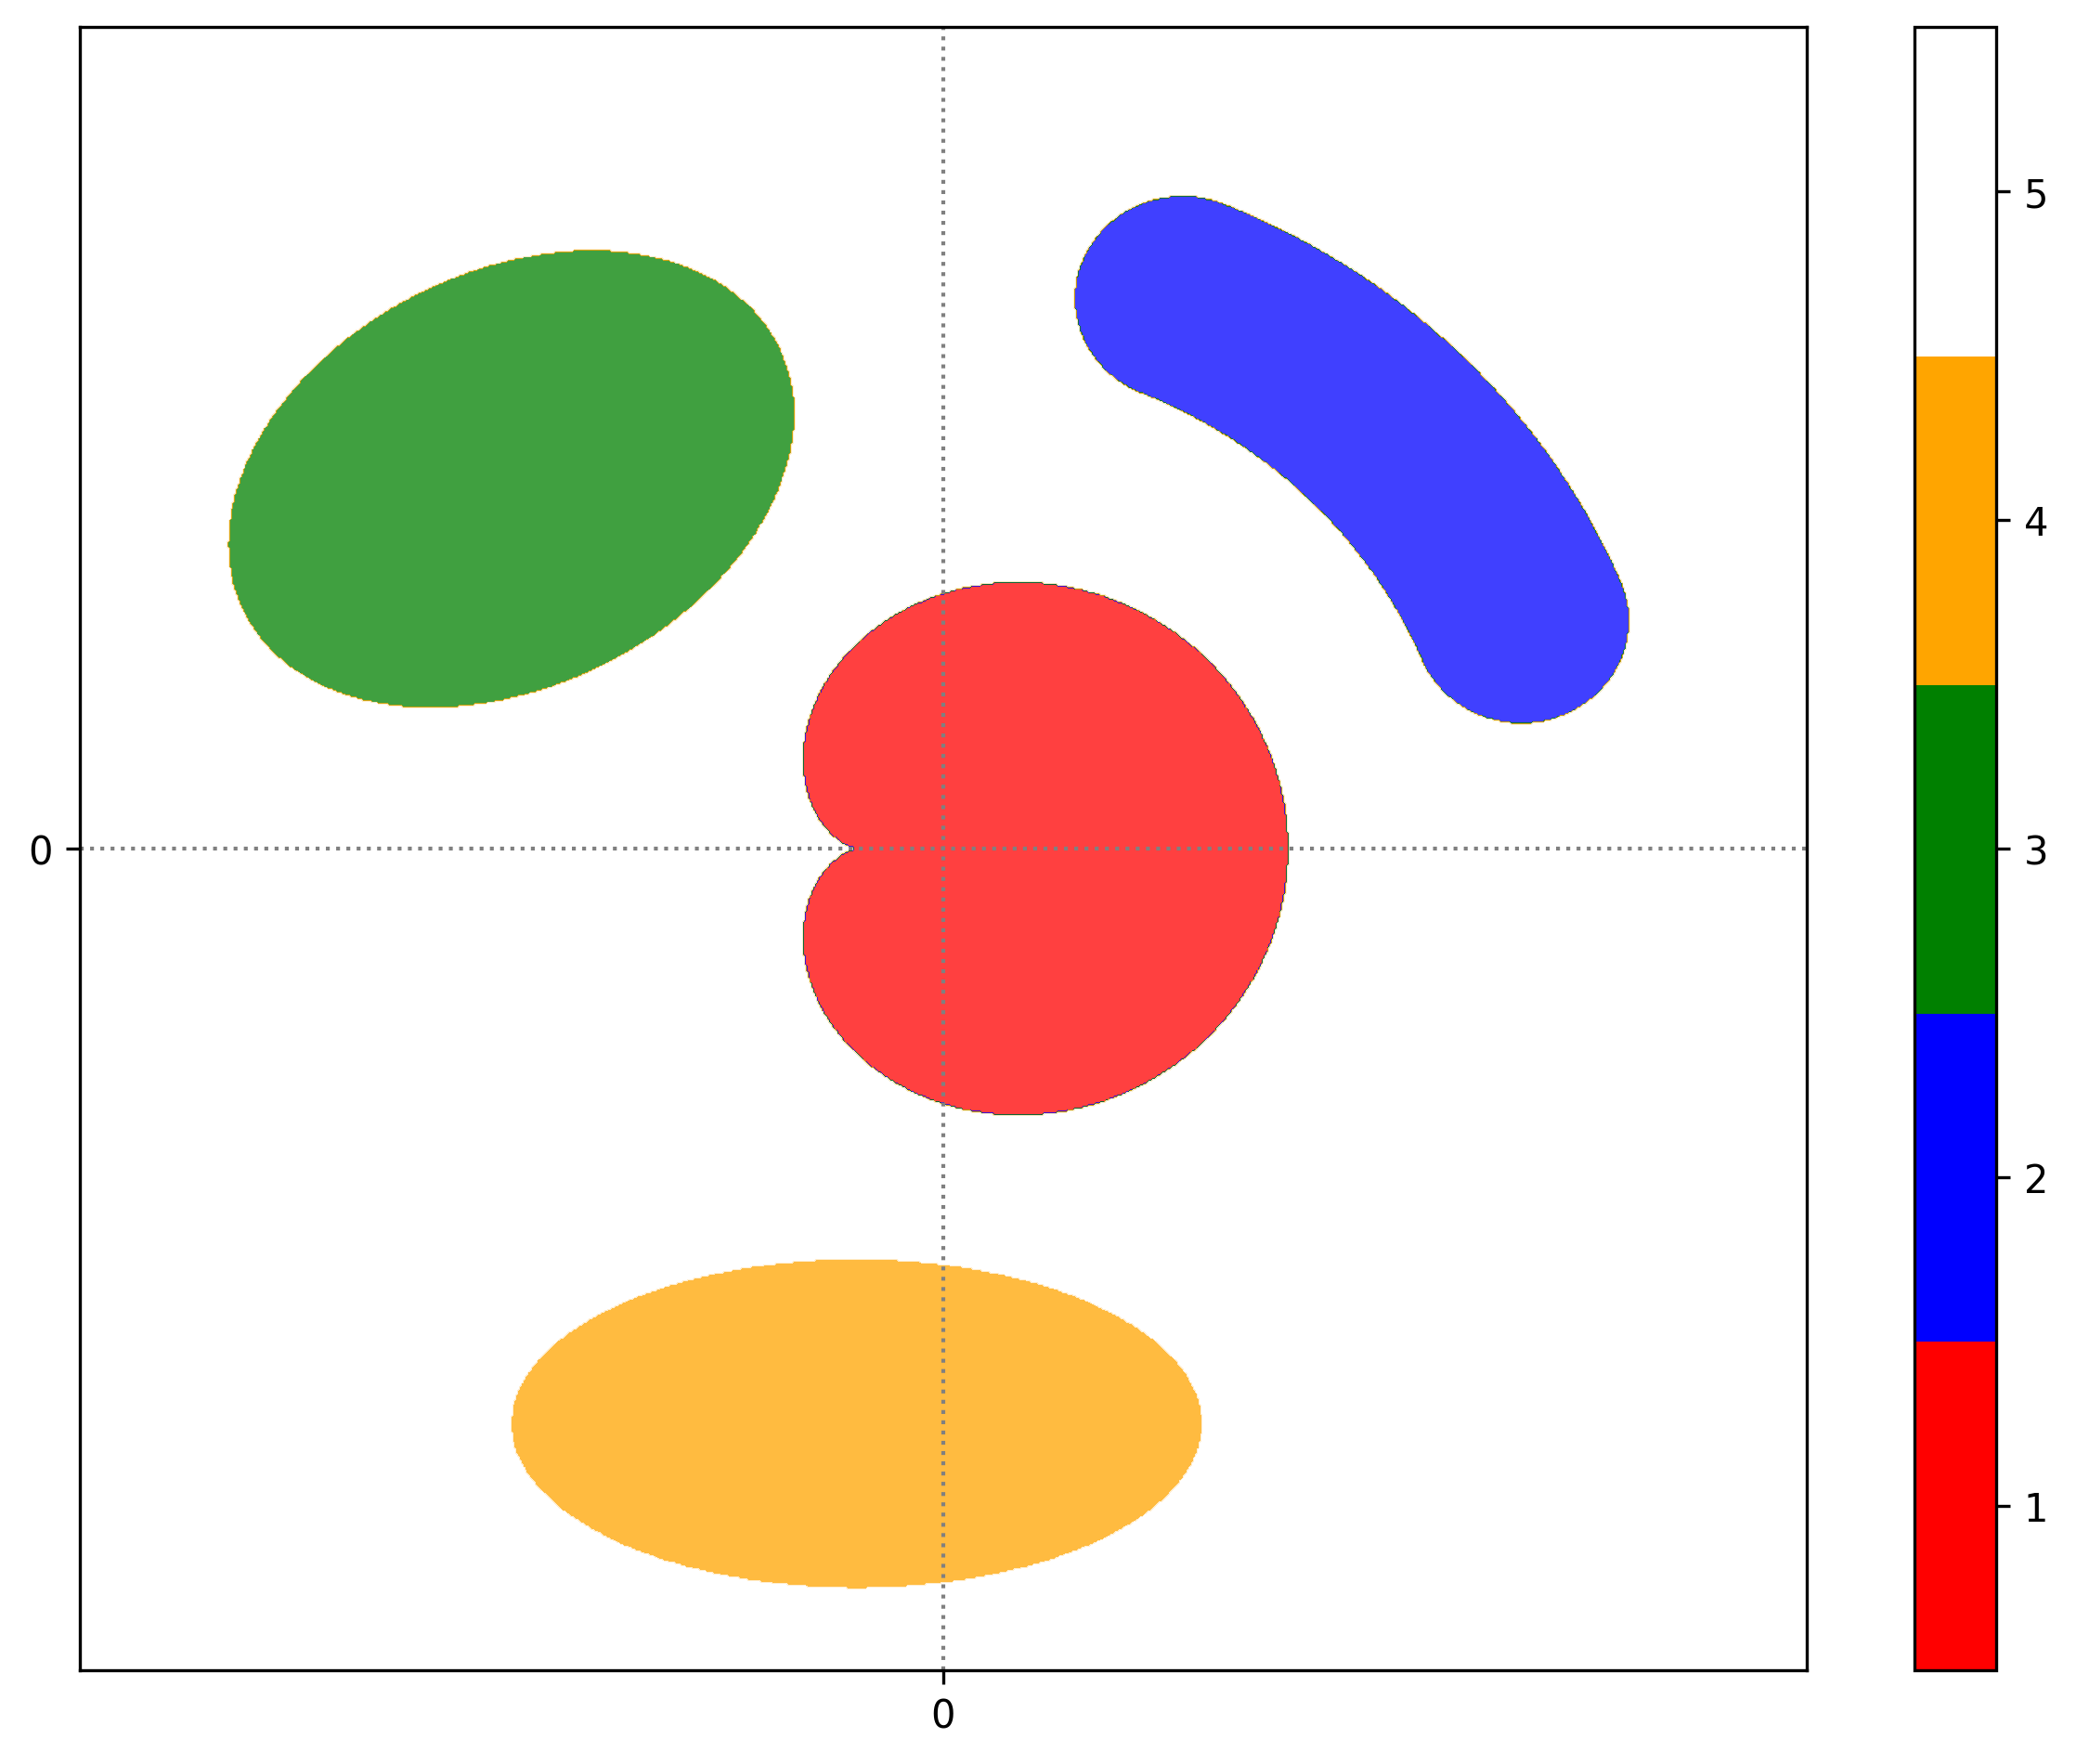
\includegraphics[height=0.35\textheight]{figures/ex1_structures.png}
	\end{center}
	\caption{Anatomical structures for \S\ref{sec:ex_simple}. Red is the target ($i = 1$), while green ($i = 2$), blue ($i = 3$), and orange ($i = 4$) are organs-at-risk. White denotes the body voxels ($i = 5$).}
	\label{fig:ex1_structs}
\end{figure}

The health status of the target represents the size of the tumor, while the health status for the organs-at-risk represents the amount of cell damage due to radiation or disease. Initially, the status is $h_0 = [1,0,0,0,0]$, and it evolves linearly according to equation (\ref{eq:health_dyn_linear}) with
\begin{align*}
	F_t &= \phantom{+}\diag([1.05, 0.90, 0.75, 0.80, 0.95]), \\
	G_t &= -\diag([0.01, 0.50, 0.25, 0.15, 0.0075]), \\
	r_t &= 0.
\end{align*}
% \[
%	F_t = \left(\begin{array}{ccccc}
%		1.05 & 0 & 0 & 0 & 0 \\
%		0 & 0.90 & 0 & 0 & 0 \\
%		0 & 0 & 0.75 & 0 & 0 \\
%		0 & 0 & 0 & 0.80 & 0 \\
%		0 & 0 & 0 & 0 & 0.95
%	\end{array}\right),
% \]
% \[
%	G_t = \left(\begin{array}{ccccc}
%		-0.01 & 0 & 0 & 0 & 0 \\
%		0 & -0.50 & 0 & 0 & 0 \\
%		0 & 0 & -0.25 & 0 & 0 \\
%		0 & 0 & 0 & -0.15 & 0 \\
%		0 & 0 & 0 & 0 & 0.0075
%	\end{array}\right),
% \]
% and $r_t = 0$.
We can think of $(F_t)_{ii}$ as the growth/regeneration rate and $(G_t)_{ii}$ as the radiation damage rate of structure $i$. For the health penalty function, we choose $\psi_t(h_t) = \|h_t\|_2^2$. The health trajectory is constrained to lie within the bounds
\begin{align*}
	H_t^{\min} &= -[0, 0.5, 0.5, 0.95, 1.25], \quad H_t^{\max} = [1.50, 0, 0, 0, 0], \quad t = 1,\ldots,15, \\
	H_t^{\min} &= -[0, 0.5, 0.5, 0.95, 1.25], \quad H_t^{\max} = [0.05, 0, 0, 0, 0], \quad t = 16,\ldots,20.
\end{align*}

With $\rho = 1$, ADMM converged in 61 iterations using cutoffs of $\epsilon_{\text{abs}} = 10^{-6}$ and $\epsilon_{\text{rel}} = 10^{-3}$. The optimal treatment plan is depicted in Figure \ref{fig:ex1_beams}. Beams are densely clustered diagonal from the vertical, striking the target while largely sparing the sensitive organs-at-risk $i=2,3$. As the sessions continue, their intensity drops off so that over half the initial beams are disabled by $t=10$. Subsequently, treatment remains constant until $t=16$ -- when the target's health bound becomes more stringent -- after which only a single low-intensity beam remains, maintaining the desired health status.  %, directed solely at the target and intervening body voxels.

Figure \ref{fig:ex1_traj} shows the radiation dose and health status resulting from this plan. Total dose to the target ($i=1$) and body voxels ($i=5$) far exceed the dose to other structures. By the end of treatment, the target's health status has fallen to a steady 0.05, while the health of the organs-at-risk remain within their respective lower limits.

\begin{figure}
	\begin{center}
		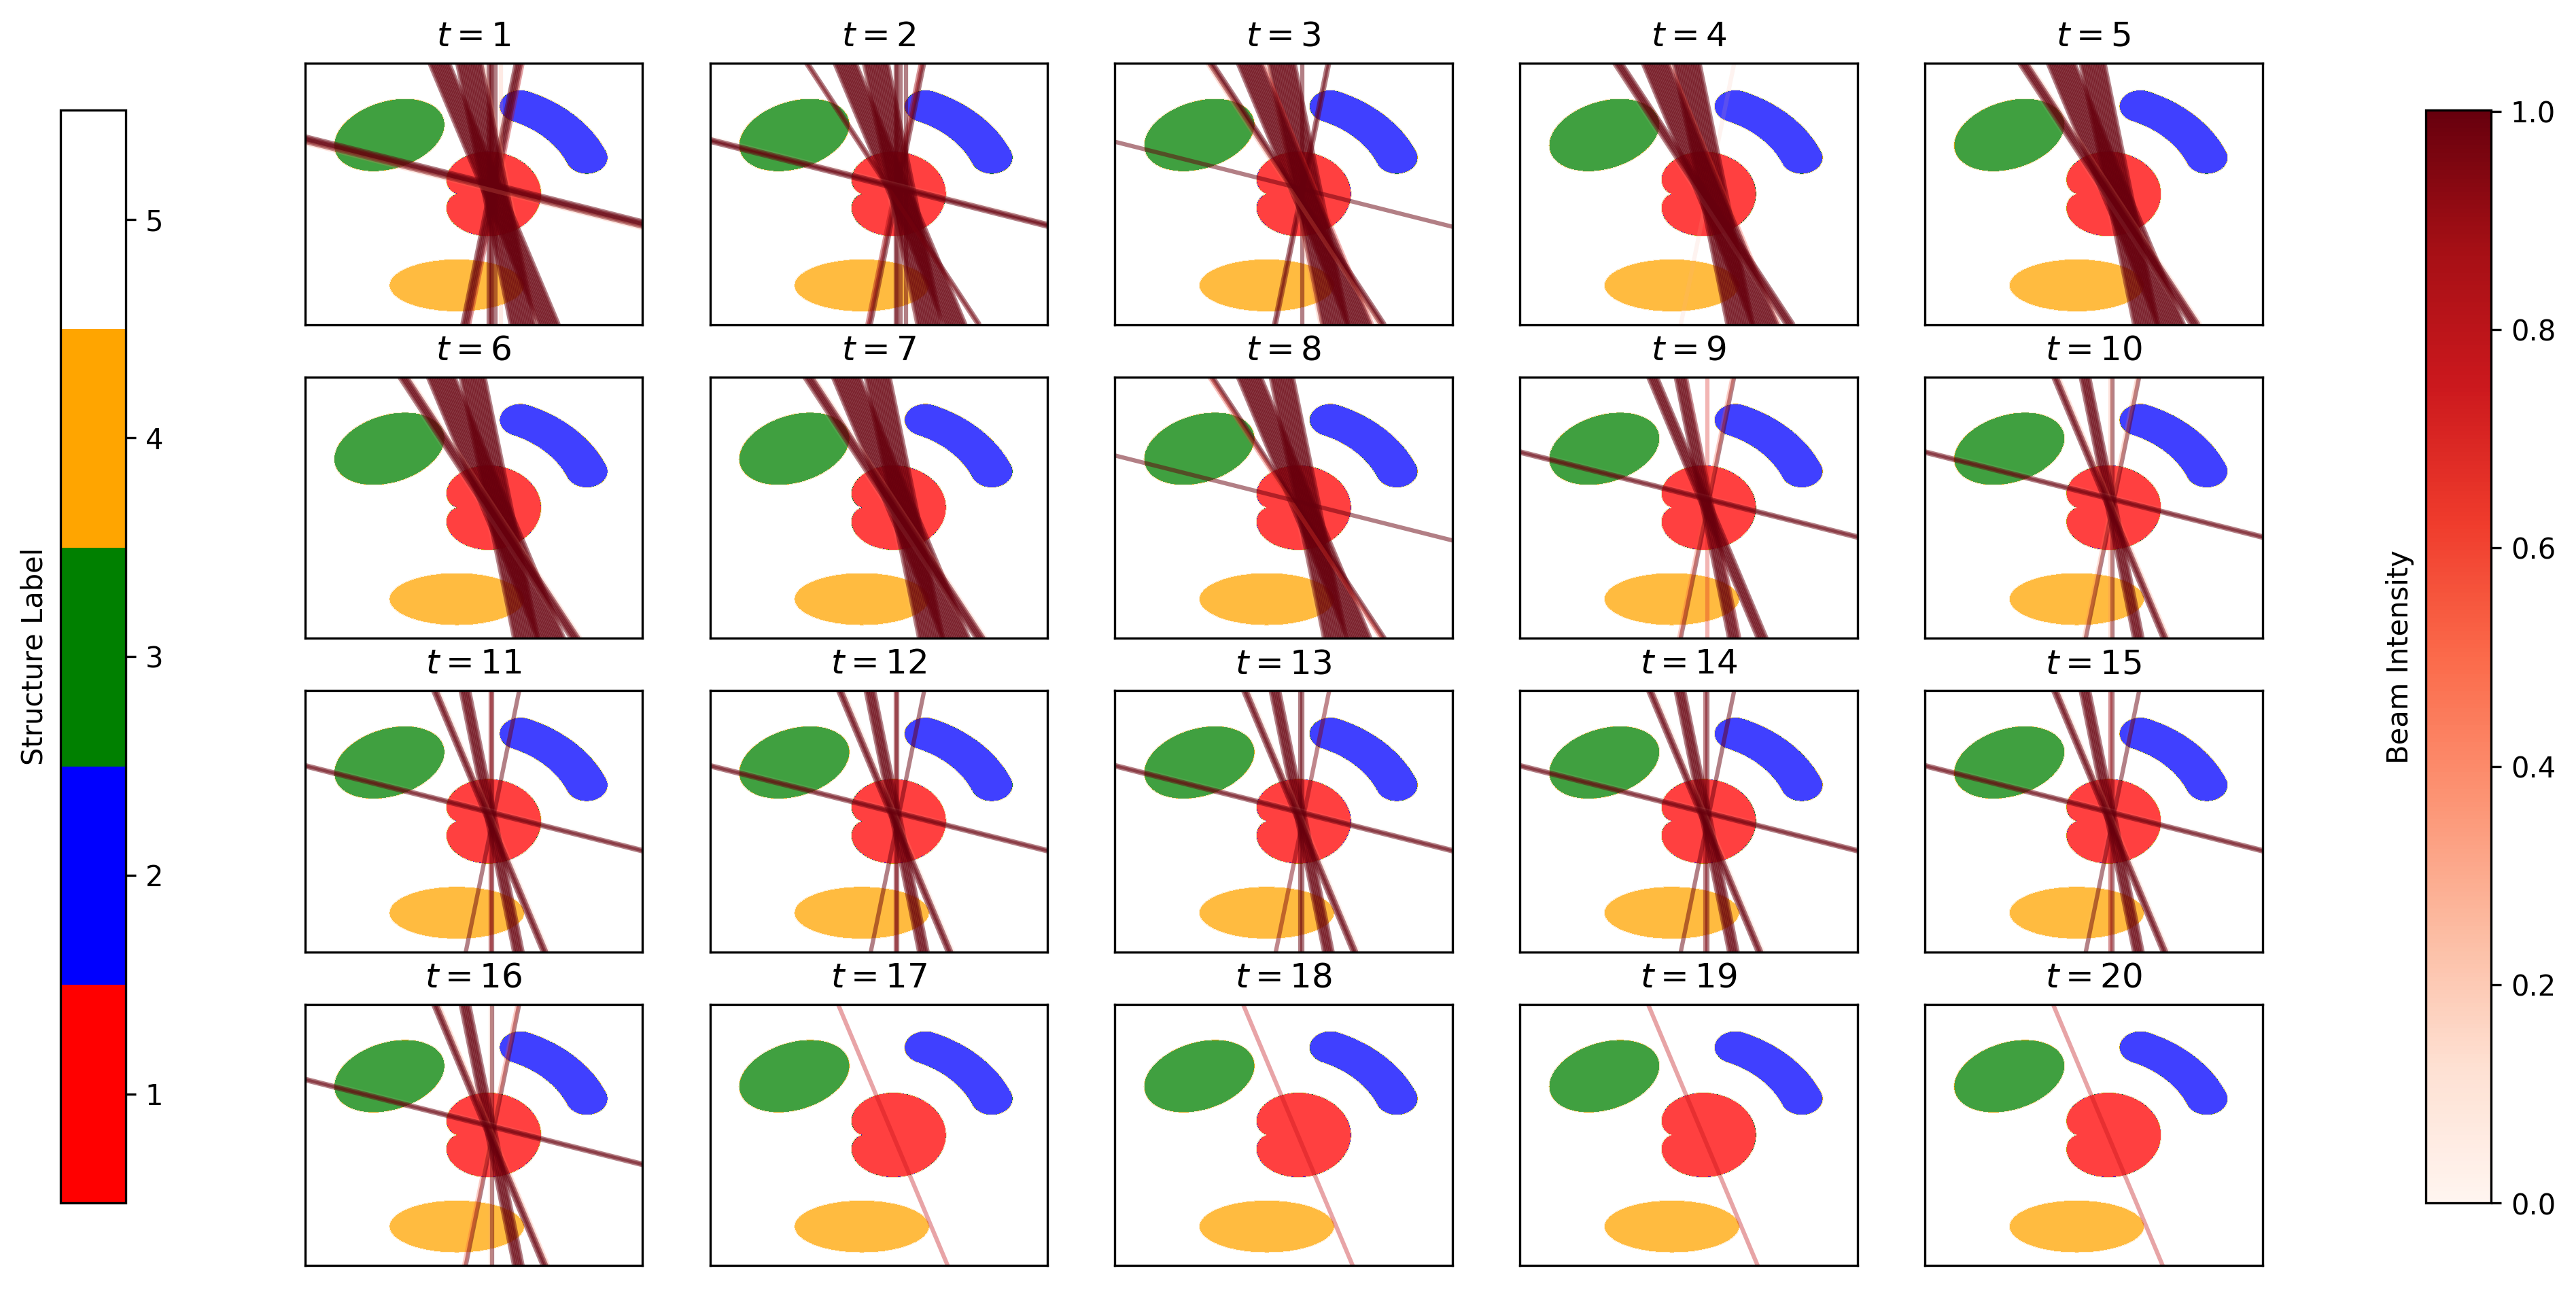
\includegraphics[width=0.95\textwidth]{figures/ex1_beams.png}
	\end{center}
	\caption{Optimal beam intensities for \S\ref{sec:ex_simple}.}
	\label{fig:ex1_beams}
\end{figure}

\begin{figure}
	\begin{center}
		\begin{subfigure}[b]{0.95\textwidth}
			\caption{Dose Trajectories}
			\label{fig:ex1_traj_dose}
			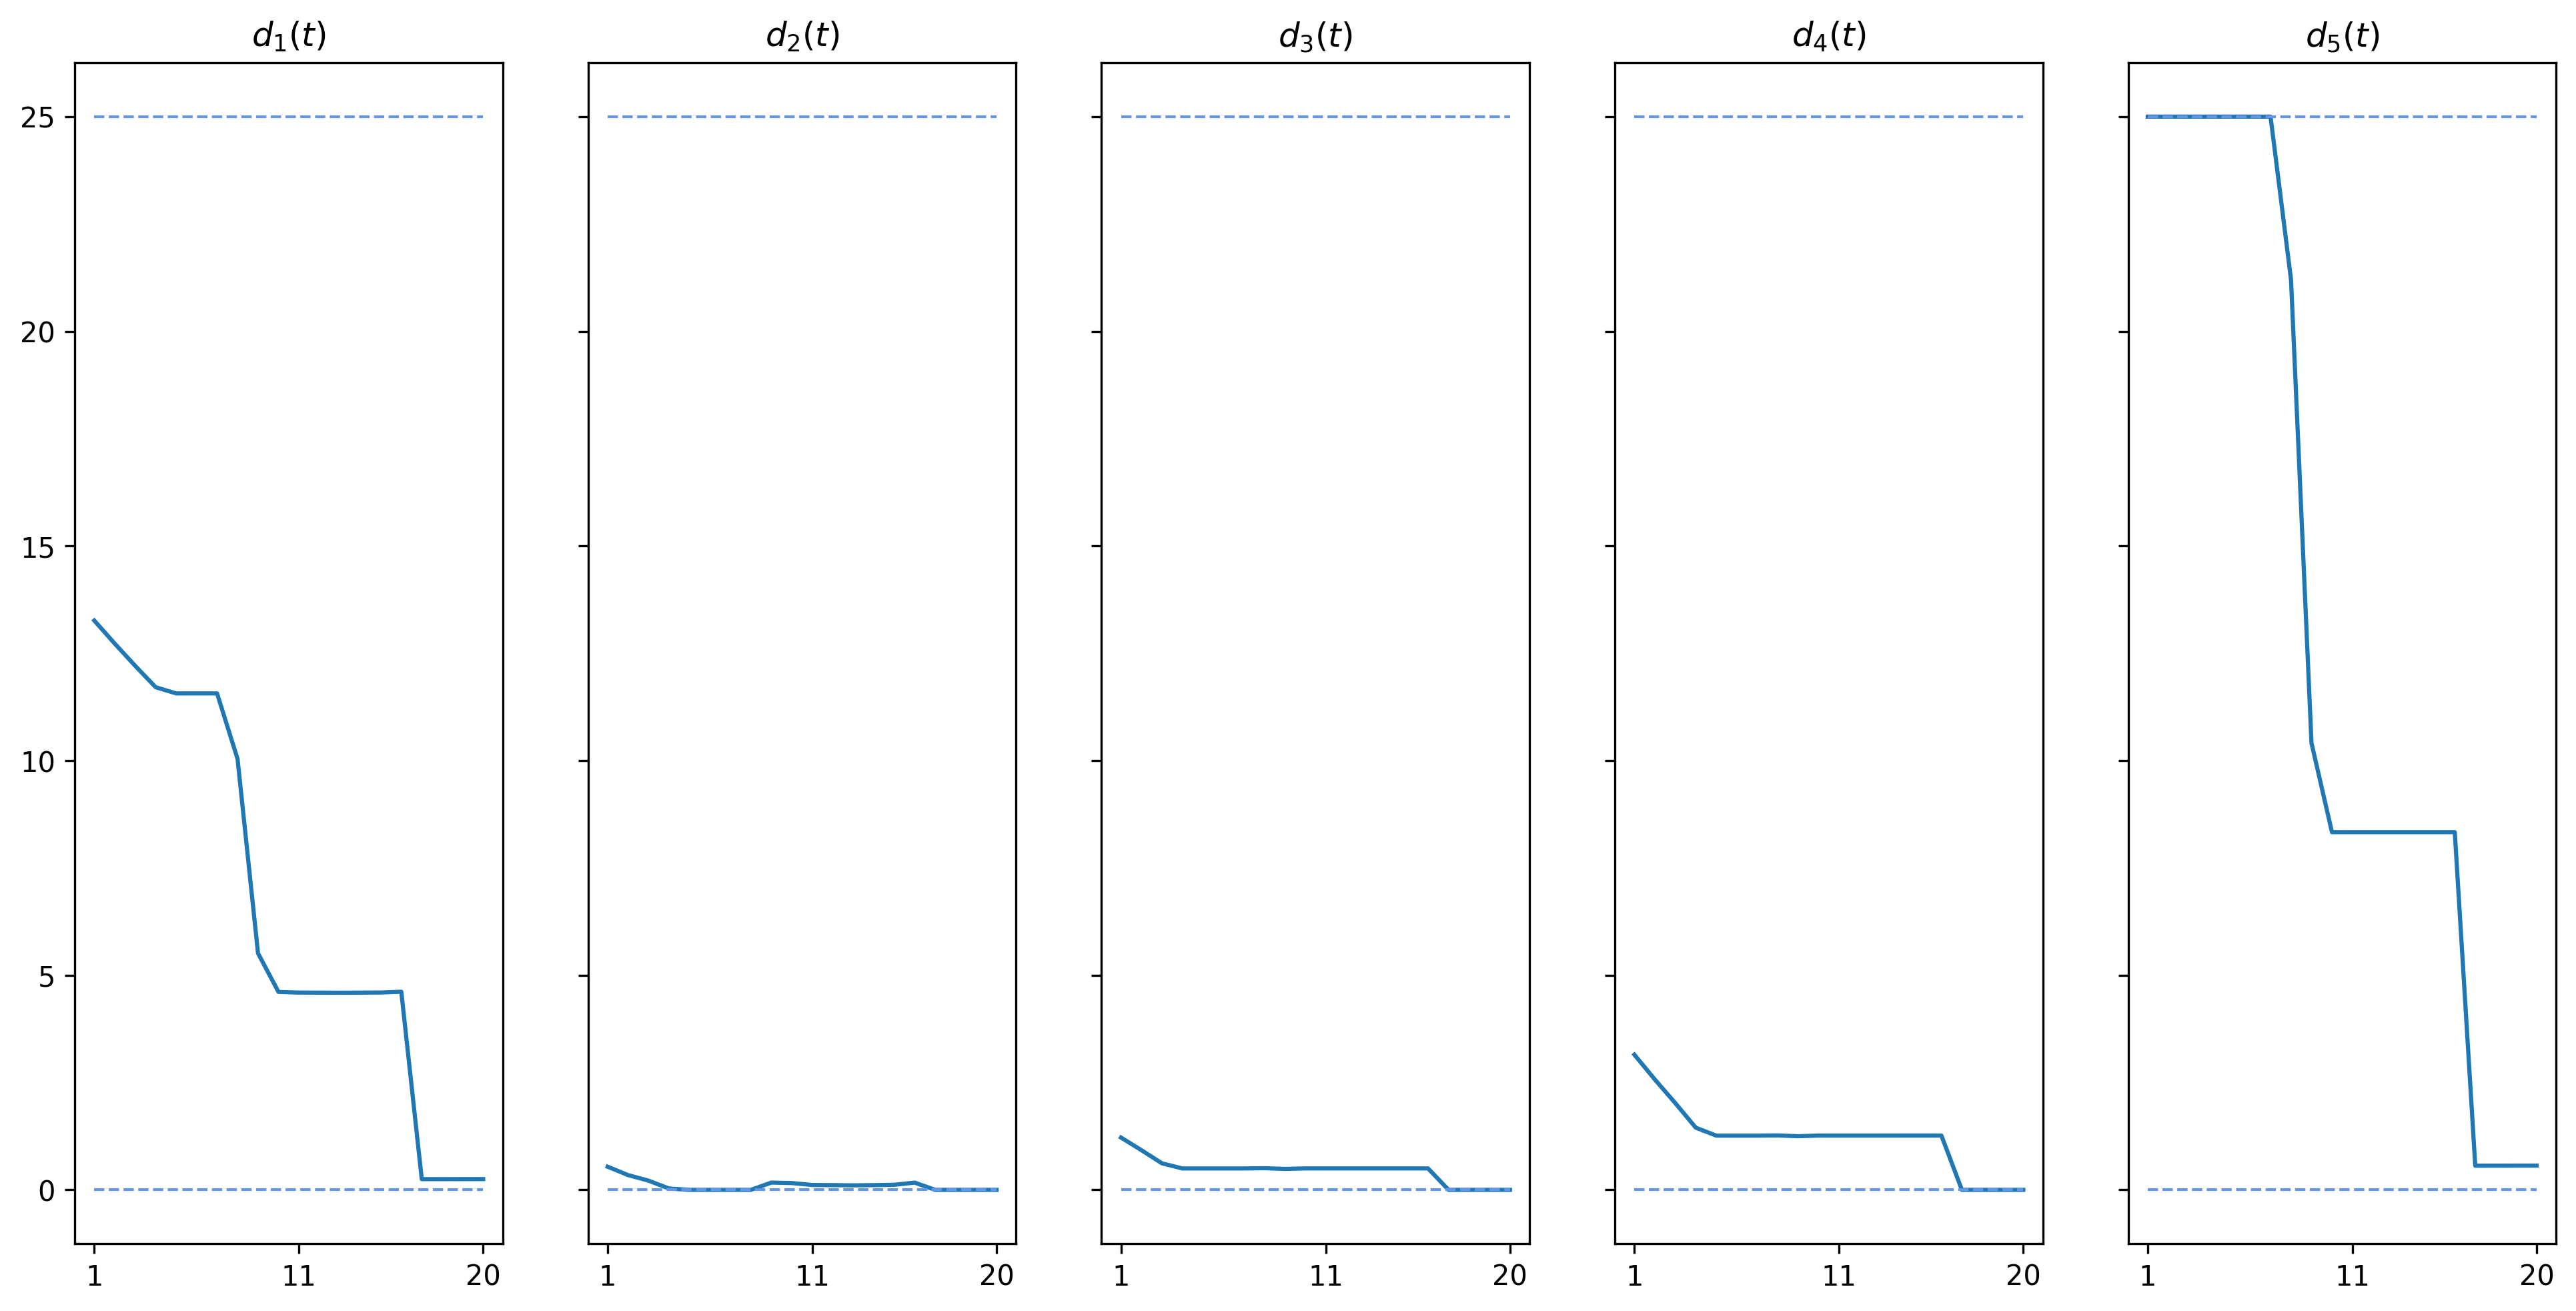
\includegraphics[width=\textwidth]{figures/ex1_doses.png}
		\end{subfigure}
		\par\bigskip
		\begin{subfigure}[b]{0.95\textwidth}
			\caption{Health Trajectories}
			\label{fig:ex1_traj_health}
			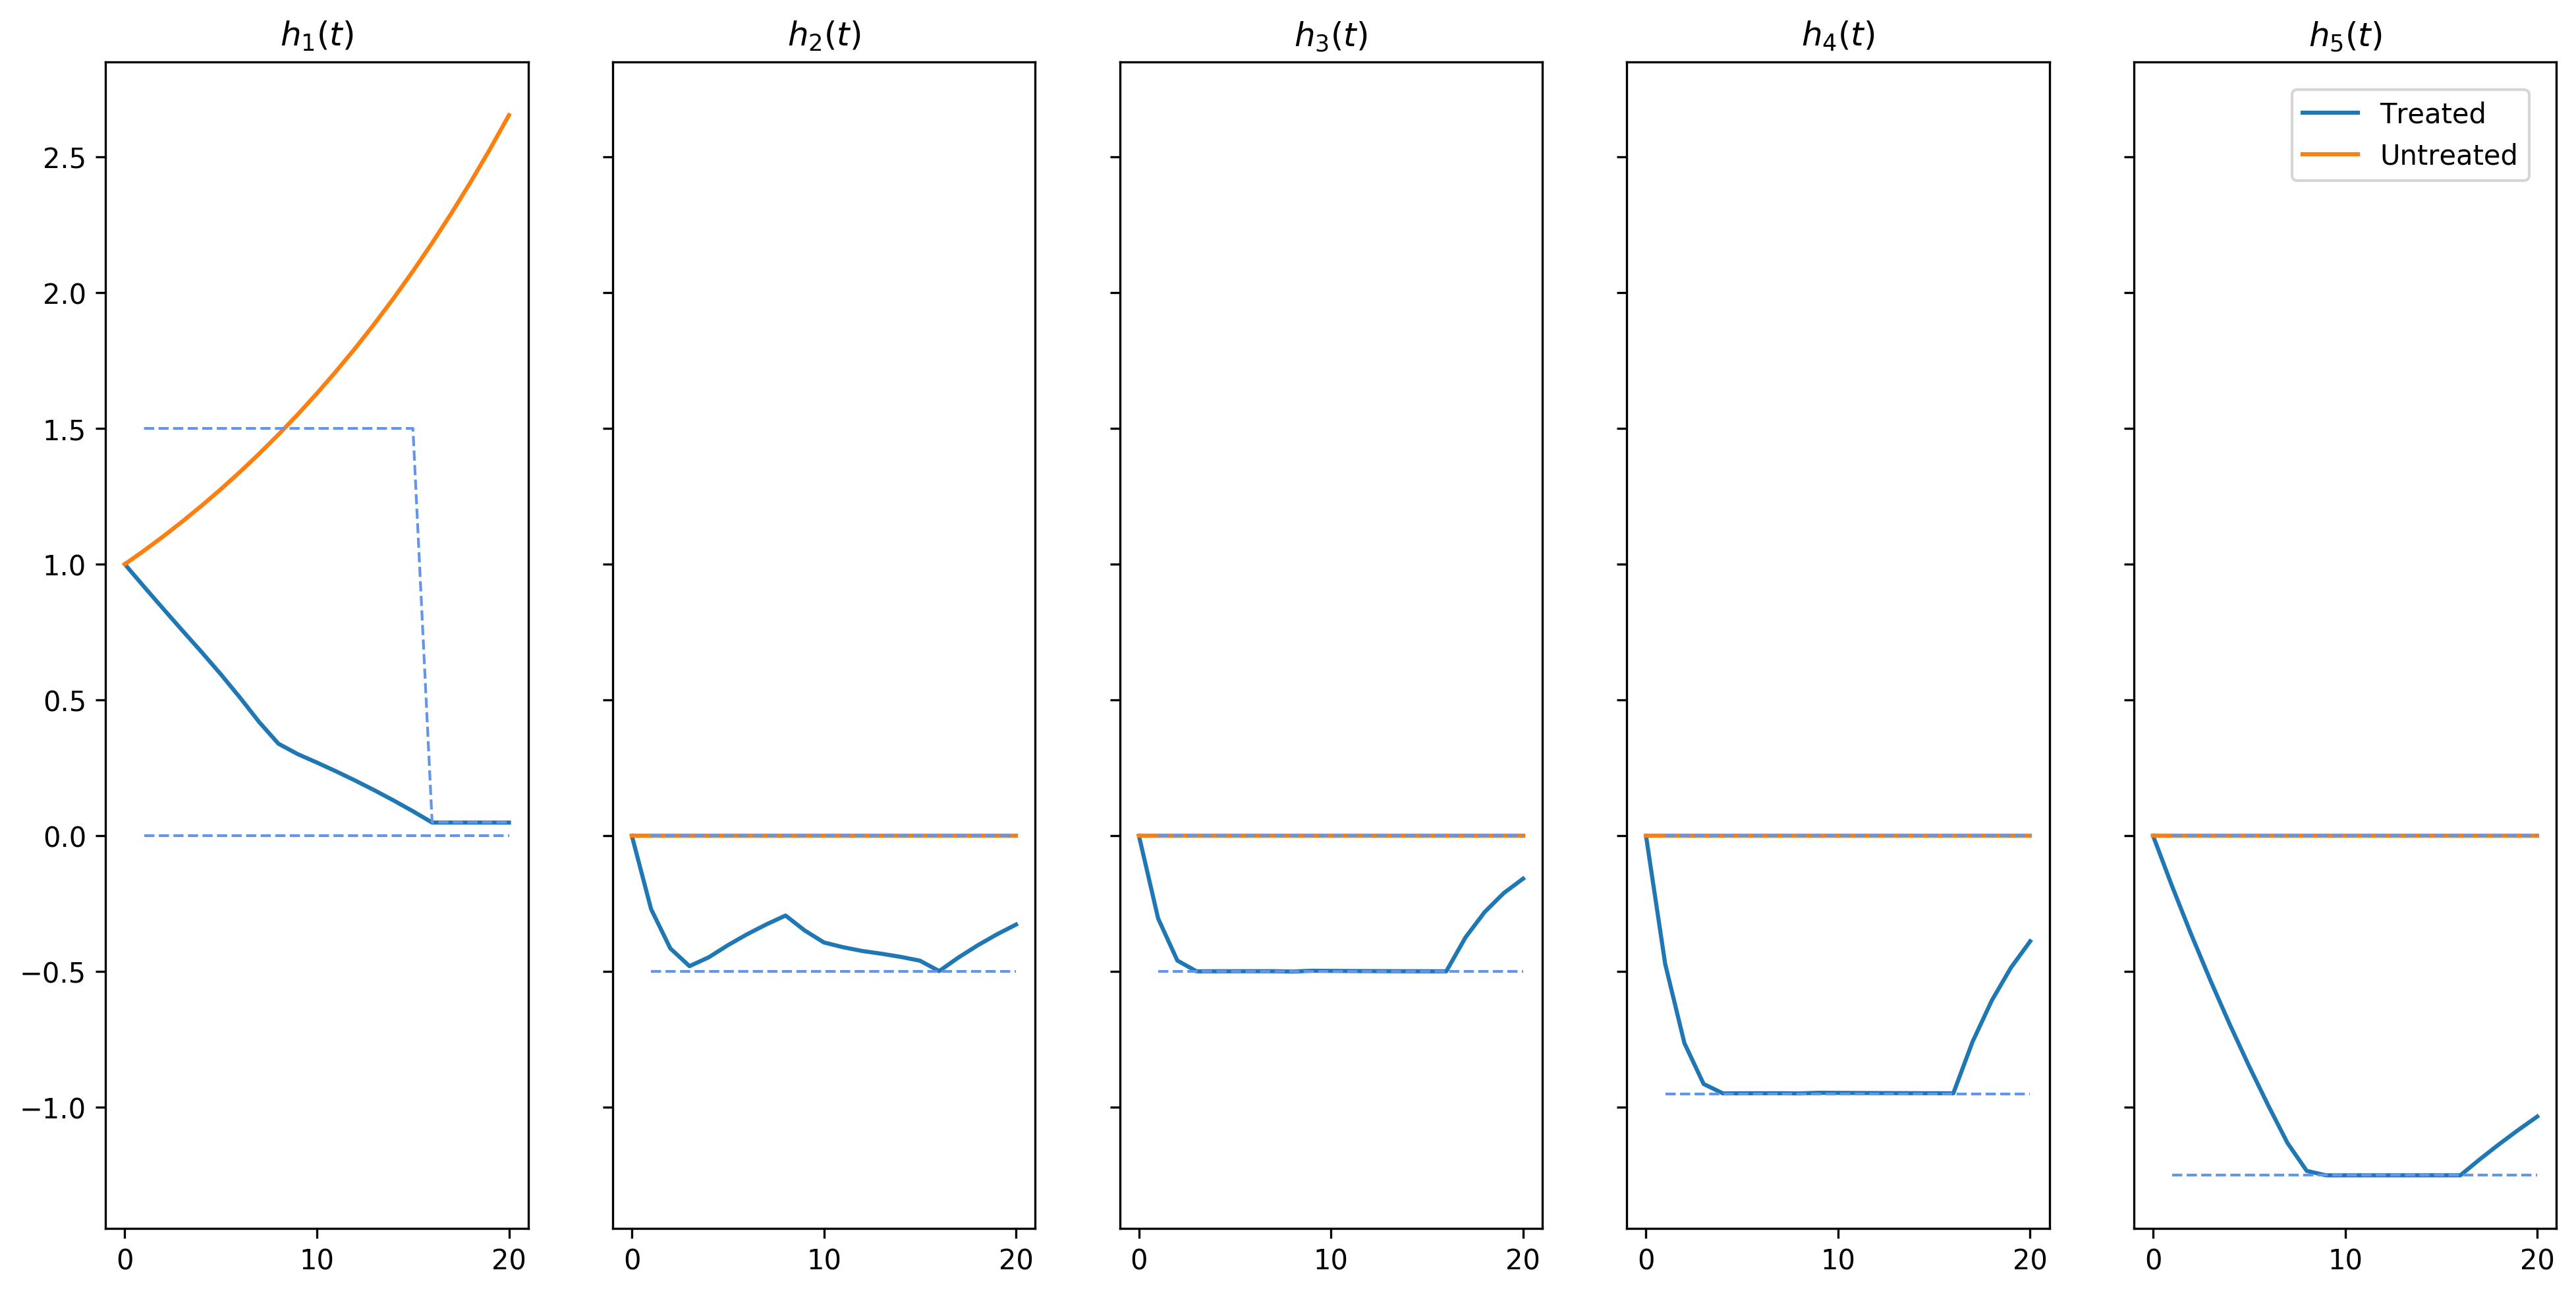
\includegraphics[width=\textwidth]{figures/ex1_health.png}
		\end{subfigure}
		\caption{Optimal (a) radiation dose and (b) health status trajectories for \S\ref{sec:ex_simple}.}
		\label{fig:ex1_traj}
	\end{center}
\end{figure}

\subsection{Prostate FMO Example}
\label{sec:ex_prostate}
% Example for scalability.

\section{Model Predictive Control}
\label{sec:mpc}
So far, we have assumed that at the time of planning, our model $f_t$ perfectly captures the health dynamics for $t=1,\ldots,T$.
% our models of the dose physics and health dynamics are perfectly accurate for $t=1,\ldots,T$. % $A_t$ and $f_t$ are perfectly known for $t=1,\ldots,T$.
This is rarely true in practice. A patient's anatomy changes unpredictably between sessions, altering the dispersion of radiation beams and the course of the health trajectory. We can incorporate these changes into our problem using model predictive control (MPC). % We deal with these uncertainties using model predictive control (MPC).

MPC is a powerful technique for automatic control of complex, nonlinear, stochastic systems. 
% It is especially fitting for radiation treatment because the patient's health and anatomy are reassessed at the beginning of each session, allowing changes to be rapidly incorporated into the solution. 
It performs extremely well even when the dynamics are approximated by a simple model, since the system's state is updated regularly and new information incorporated into the solution. This is particularly fitting for radiation treatment planning. % because the patient's health and anatomy are reassessed at the beginning of each session.

At the beginning of session $t$, we observe $A_t, f_t$, and the patient's true health status, $h_{t-1}$. Then, we solve the problem
% A standard approach to problem (\ref{prob:dyn_single}) is model predictive control (MPC) with a shrinking time horizon \cite{CamachoBordons:2007}. 
\BEQ
\label{prob:dyn_single_mpc}
\begin{array}{lll}
	\mbox{minimize} & \sum_{\tau=t}^T \phi_{\tau}(d_{\tau}) + \sum_{\tau=t}^T \psi_{\tau}(h_{\tau}) & \\
	\mbox{subject to} & b_{\tau} \geq 0, \quad d_{\tau} = A_t b_{\tau}, \quad 0 \leq d_{\tau} \leq D_{\tau}^{\max}, \quad & \tau = t,\ldots,T, \\
	& h_{\tau} = f_t(h_{\tau-1}, d_{\tau}), \quad H_{\tau}^{\min} \leq h_t \leq H_{\tau}^{\max}, \quad & \tau = t,\ldots,T
\end{array}
\EEQ
with variables $(b_t,\ldots,b_T), (d_t,\ldots,d_T)$, and $(h_t,\ldots,h_T)$. This can be done using a slight variation of Algorithm \ref{algo:admm}. Let the resulting treatment plan be $\bar b = (\bar b_t,\ldots, \bar b_T)$. We carry out only the first treatment, $\bar b_t$, and update our observations before the next session, % reassess the patient in the next session, 
repeating until all $T$ sessions have been completed.
% Problem (\ref{prob:dyn_single}) is convex and may be solved using MPC with general convex solvers \cite{KimPhillips:2012}.

TODO: Introduce slack problem.

\subsection{Illustrative Example with MPC}
\label{sec:ex_simple_mpc}
We return to the setting of \S\ref{sec:ex_simple}, except now, the health dynamics are modeled with some error. % the health dynamics model contains some uncertainty/error.
% Specifically, the patient's true health status at the start of session $t$ is
% \[
%	h_{t-1} = \begin{cases}
%		h_0 & t = 1 \\
%		f_{t-1}(h_{t-2},d_{t-1}) + \omega_{t-1} & t = 2,\ldots,T,
%	\end{cases}
% \]
% where each $\omega_{t-1} \in \reals^K$ is % drawn from a truncated Gaussian distribution -- we sample 
% calculated by drawing $\hat \omega_1,\ldots,\hat \omega_K$ IID from $N(0,0.025)$ and letting
% \[
%	(\omega_{t-1})_i = \begin{cases}
%		\max(\hat \omega_i,0) & i \in \mathcal{T} \\
%		\min(\hat \omega_i,0) & i \notin \mathcal{T}.
%	\end{cases}
% \]
% This ensures that the status of the target (organs-at-risk) is always nonnegative (nonpositive).
Specifically, let $h_{t-1}$ be the patient's health status at the beginning of session $t$ and $d_t$ the dose delivered during this session. Our model predicts the status will become $\hat h_t = f_t(h_{t-1},d_t)$. In fact, at the beginning of session $t+1$, we observe the true health status to be
\[
	(h_t)_i = \begin{cases}
		\max(\hat h_t + \omega_t, 0)_i & i \in \mathcal{T} \\
		\min(\hat h_t + \omega_t, 0)_i & i \notin \mathcal{T},
	\end{cases}
\]
where $\omega_t \in \reals^K$ is drawn from $N(\mu,\sigma^2I)$. This random process continues for $t = 1,\ldots,T-1$. 

For this example, we use $\mu = 0$ and $\sigma = 0.05$; all other values are identical to \S\ref{sec:ex_simple}. In particular, we still employ the linear dynamic model (\ref{eq:health_dyn_linear}) with constant $F_t,G_t$, and $r_t$, even though the health status is now stochastic. Figure \ref{fig:ex2_mpc_beams} depicts the treatment plan determined by MPC. Most beams are aimed slightly diagonal from the vertical, similar to the naive plan (Figure \ref{fig:ex1_beams}) that is produced by solving problem (\ref{prob:dyn_single}) once at the start of treatment. At the beginning, a few also cluster around the horizontal axis, but these disappear after session 8, when the beam intensities start to thin out. All beams are turned off by session 16, and they remain off except for a brief spike in the final session. 
% Compared to the naive plan, MPC generates beams from a wider range of angles and intensities to compensate for uncertainty in the model.

% This compensatory effect can be seen in the doses as well. 
In Figure \ref{fig:ex2_mpc_traj_dose}, we plot the dose trajectories of MPC (green) and the naive plan (blue). The MPC curves are more jagged with large spikes at the beginning and end of treatment. % , where the algorithm adjusted for errors in the forecasted health status.
However, in each structure, the area under the MPC and naive dose curves remain on par.
% but throughout the middle sessions ($t = 4,\ldots,18$), they never rise above the corresponding naive curves. Thus, MPC delivers about the same amount of radiation as the naive plan, only spread across a wider range of angles to compensate for uncertainty in the health status.
Thus, we conclude that MPC delivers about the same amount of radiation as the naive plan, only spread across a wider range of beam angles/intensities, so as to compensate for uncertainty in the health dynamics model.

This strategy results in better patient health as shown in Figure \ref{fig:ex2_mpc_traj_health}. Both plans reduce the target's health status below 0.05, but only MPC consistently maintains the health status of the organs-at-risk above their lower bounds. In fact, the health of these organs under the MPC plan exceeds the health under the naive plan, often by a large margin. 
% It is especially prominent in structure 3, where $h_3^{\text{naive}}(8) = TODO < H_8^{\min} = -0.5 \leq h_3^{\text{MPC}}(8) = TODO$. If we define the average health violation to be
% \[
%	\omega(h) := \frac{1}{T}\sum_{t=1}^T \ones^T\max(h_t - H_t^{\max}, 0) + \ones^T\max(H_t^{\min} - h_t, 0),
% \]
% then the naive plan yields $\psi(h^{\text{naive}}) \approx TODO$, while MPC achieves $\omega(h^{\text{MPC}}) \approx TODO$.

\begin{figure}
	\begin{center}
		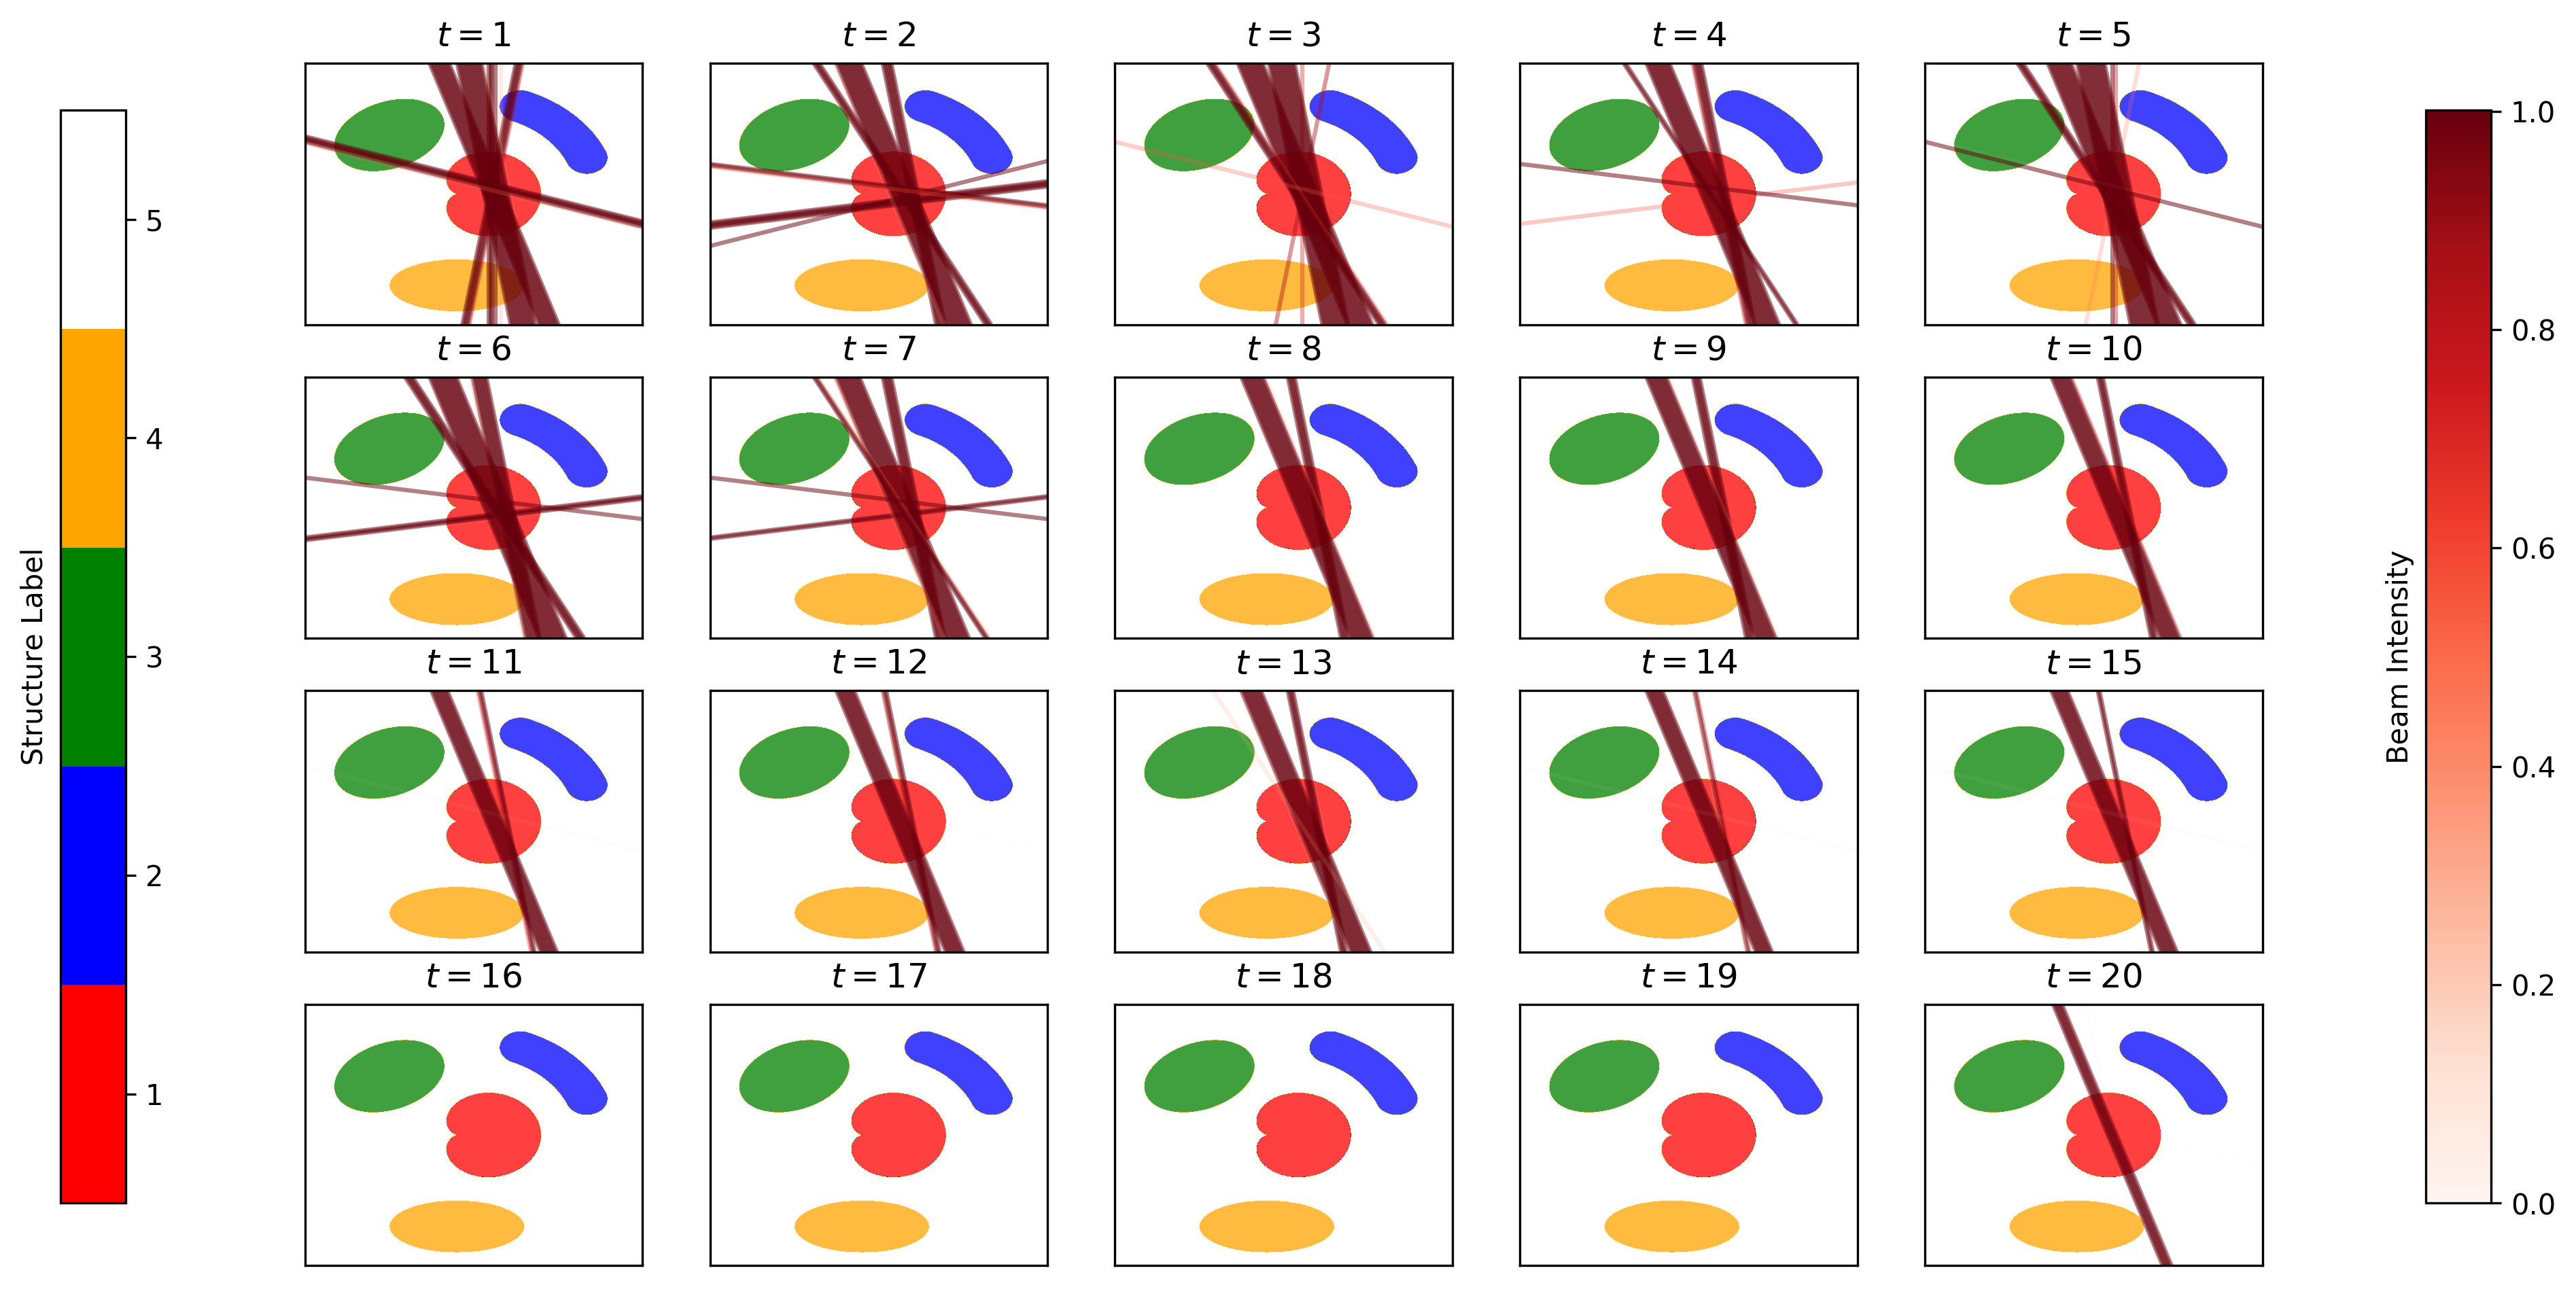
\includegraphics[width=0.95\textwidth]{figures/ex2_mpc_beams.png}
	\end{center}
	\caption{Optimal beam intensities for \S\ref{sec:ex_simple_mpc} using MPC.}
	\label{fig:ex2_mpc_beams}
\end{figure}

\begin{figure}
	\begin{center}
		\begin{subfigure}[b]{0.95\textwidth}
			\caption{Dose Trajectories}
			\label{fig:ex2_mpc_traj_dose}
			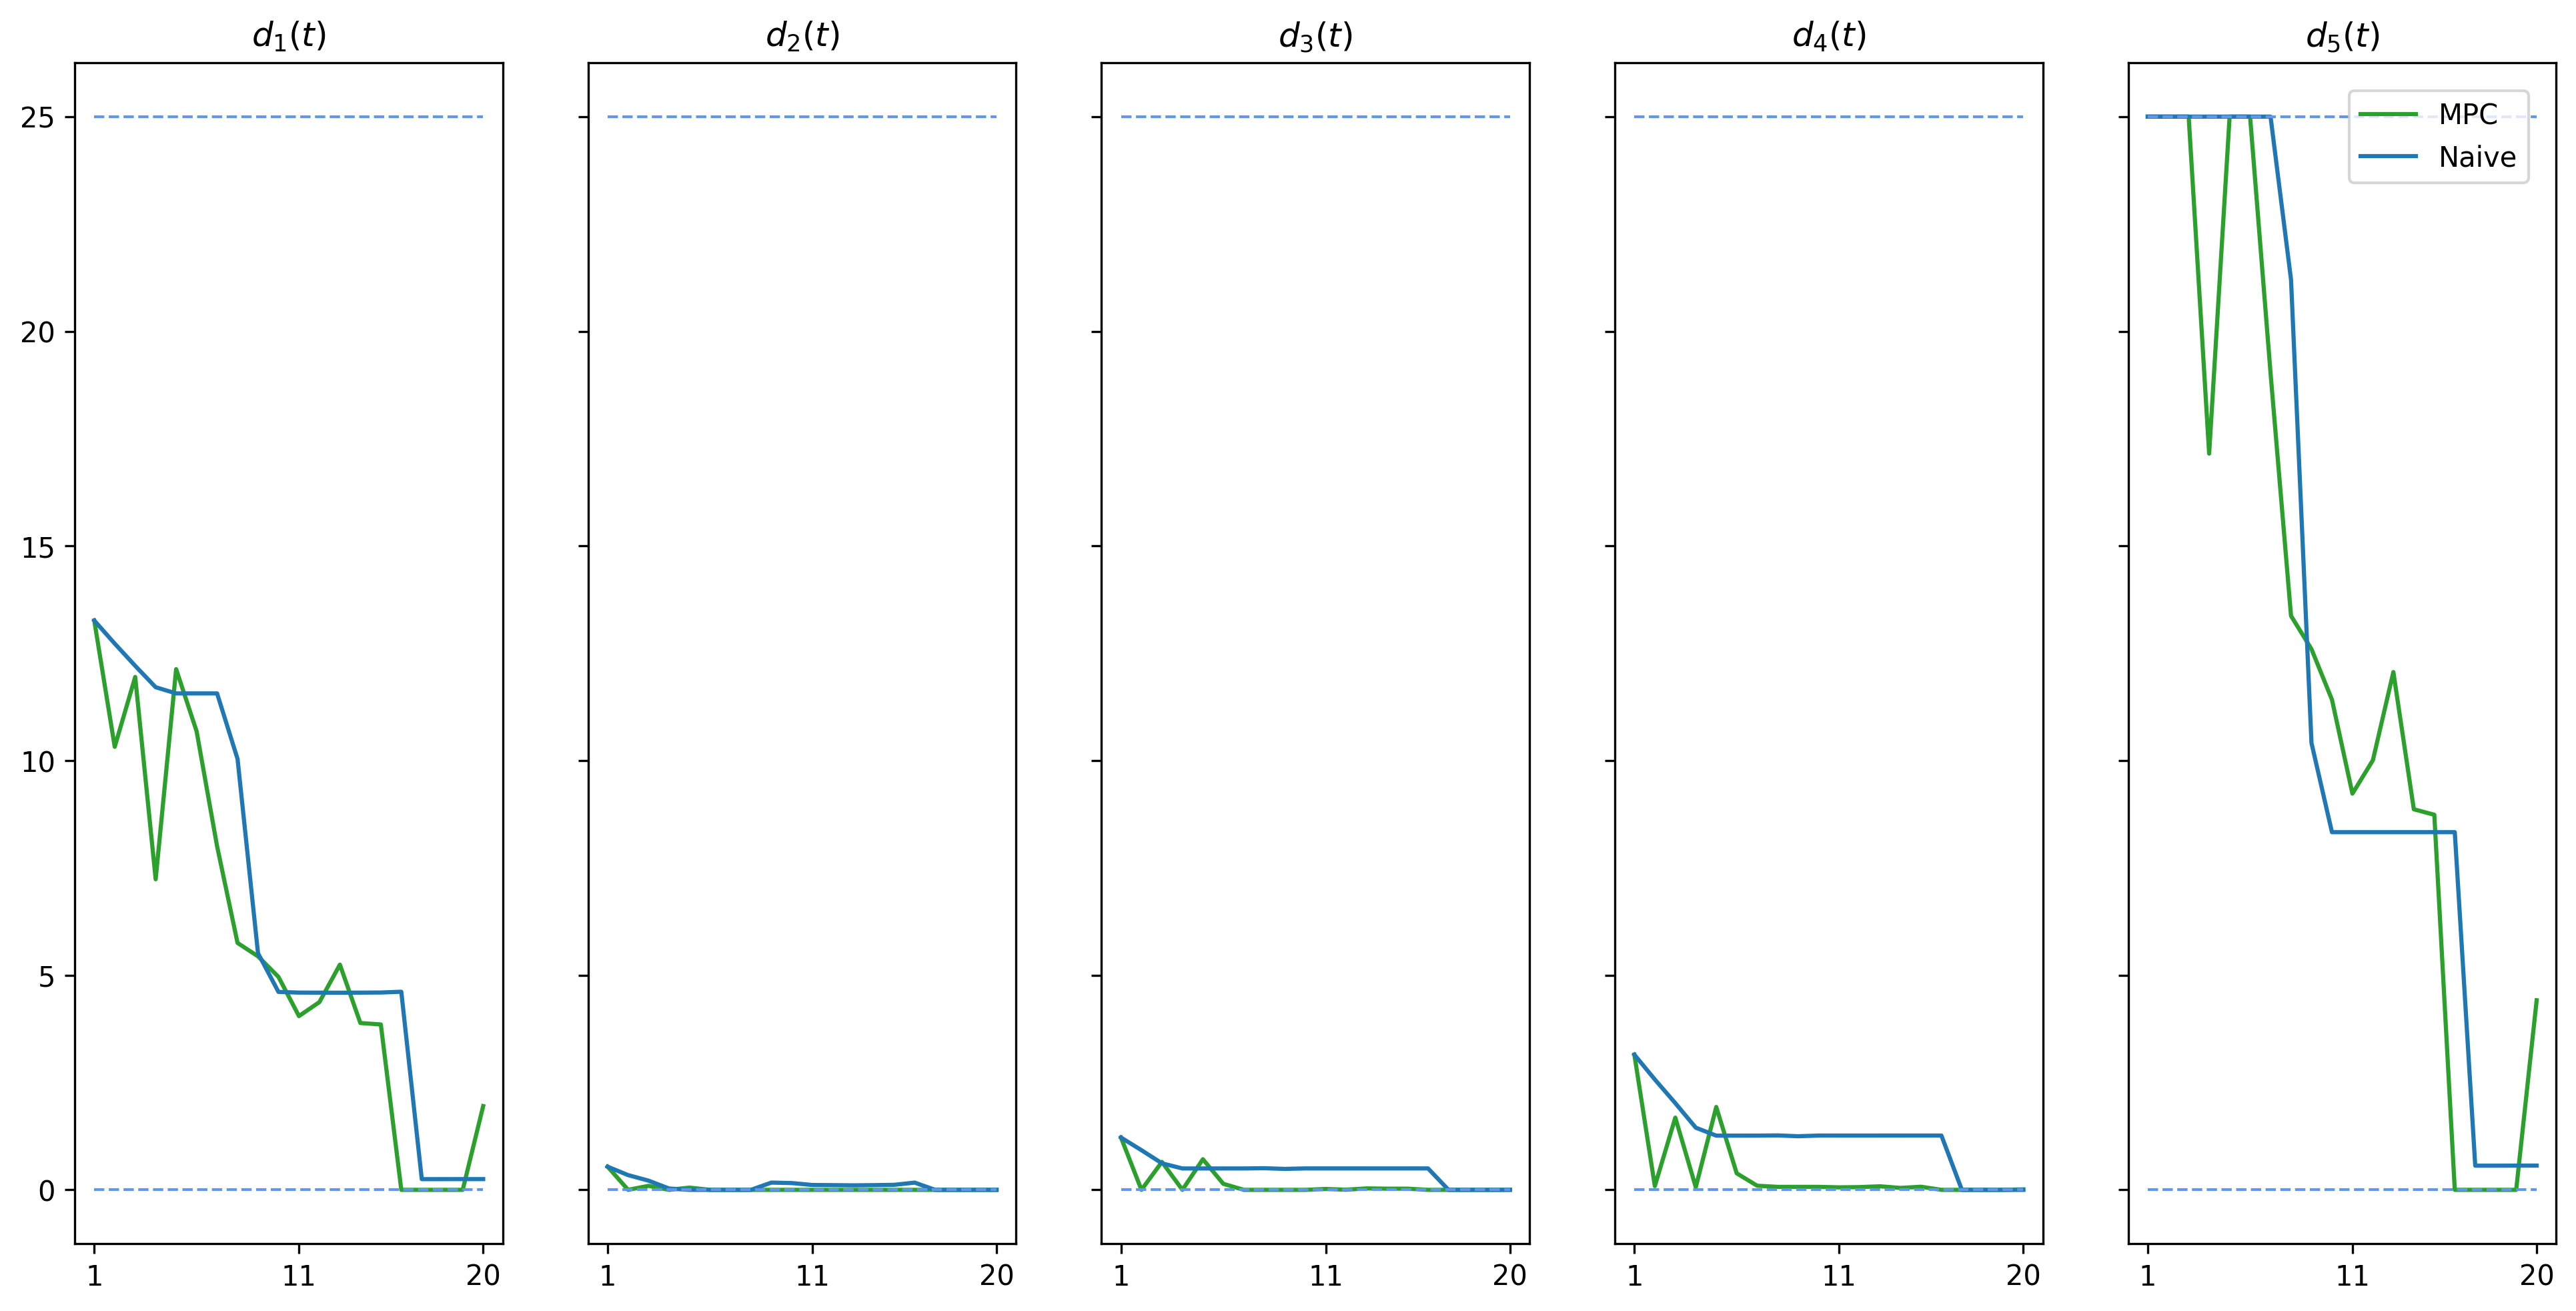
\includegraphics[width=\textwidth]{figures/ex2_mpc_doses.png}
		\end{subfigure}
		\par\bigskip
		\begin{subfigure}[b]{0.95\textwidth}
			\caption{Health Trajectories}
			\label{fig:ex2_mpc_traj_health}
			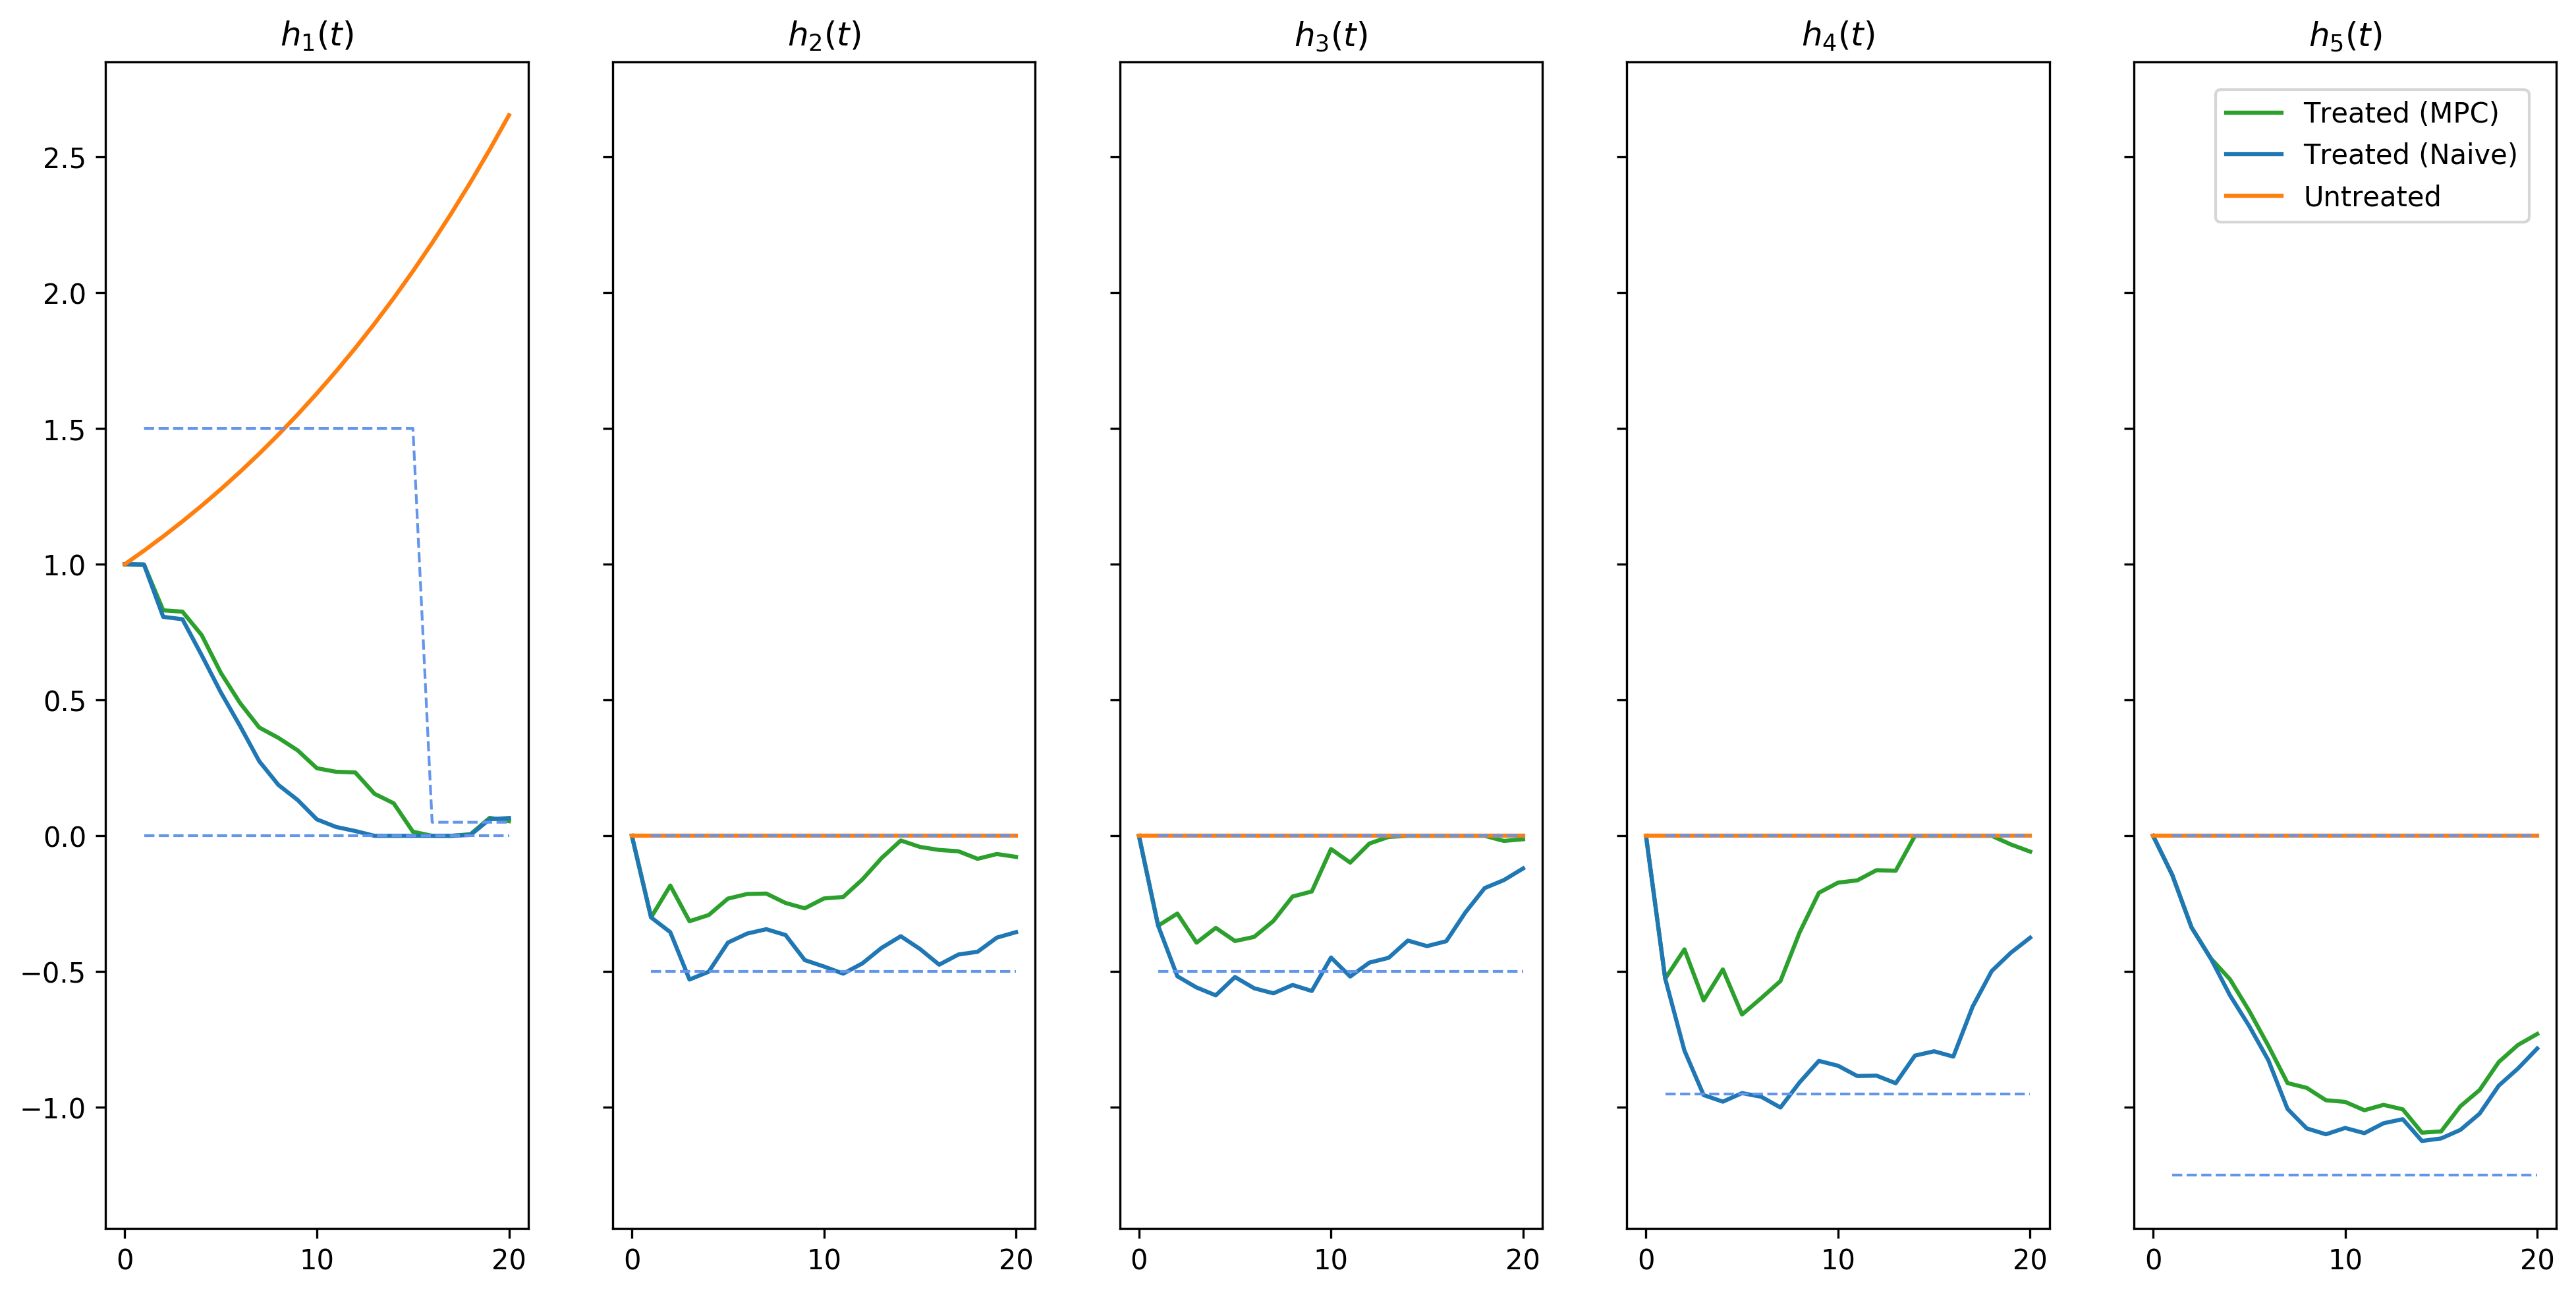
\includegraphics[width=\textwidth]{figures/ex2_mpc_health.png}
		\end{subfigure}
		\caption{Optimal (a) radiation dose and (b) health status trajectories for \S\ref{sec:ex_simple_mpc} using MPC (green) and a naive planning approach (blue). The MPC plan's health trajectories all remain within the desired bounds, despite the error in the health dynamics model.}
		\label{fig:ex2_mpc_traj}
	\end{center}
\end{figure}

\subsection{Prostate FMO Example with MPC}
\label{sec:ex_prostate_mpc}

\section{Nonlinear Health Dynamics}
\label{sec:nonlin_health}
We now consider the case when the health dynamics are nonlinear, \ie, $f_t$ is not an affine function. Nonlinear dynamics arise in many models of radiation response like the linear-quadratic model of cell survival \cite{HallGiaccia:2019}, TODO: Cite more examples.
In this case, problem (\ref{prob:dyn_single}) is nonconvex and Algorithm \ref{algo:admm} requires us to solve a nonconvex subproblem at each iteration. A variety of methods exist for approximate nonconvex optimization \cite{NocedalWright:1999} TODO: Cite more references. Here we describe one method, the convex-concave procedure.

\subsection{Convex-Concave Procedure}
\label{sec:ccp}
The convex-concave procedure (CCP) \cite{YuilleRangarajan:2003,LippBoyd:2016} is a heuristic for finding a local optimum of
\BEQ
\label{prob:ccp_gen}
	\begin{array}{ll}
		\mbox{minimize} & F_0(x) - G_0(x) \\
		\mbox{subject to} & F_i(x) - G_i(x) \leq 0, \quad i = 1,\ldots,m,
	\end{array}
\EEQ
where $x \in \reals^n$ is the variable and $F_i:\reals^n \rightarrow \reals$ and $G_i: \reals^n \rightarrow \reals$ are convex functions for $i = 0,\ldots,m$. The basic algorithm requires an initial feasible point $x^0$ of problem (\ref{prob:ccp_gen}). In each iteration $s = 1,2,\ldots$, it forms the linearization
\[
	\hat G_i(x;x^s) = G_i(x^s) + \gamma_i^T(x - x^s), \quad \gamma_i \in \partial G_i(x^s), \quad i = 0,\ldots,m
\]
and sets $x^{s+1}$ to be the solution of
\[
	\begin{array}{ll}
	\mbox{minimize} & F_0(x) - \hat G_0(x;x^s) \\
	\mbox{subject to} & F_i(x) - \hat G_i(x;x^s) \leq 0, \quad i = 1,\ldots,m.
	\end{array}
\]
This problem is convex because $F_i$ are convex and $\hat G_i(\cdot;x^s)$ are affine, so it can be solved efficiently. The iterations continue until a stopping criterion is reached, \eg,
\[
	(F_0(x^s) - G_0(x^s)) - (F_0(x^{s+1}) - G_0(x^{s+1})) \leq \delta
\]
for some $\delta > 0$. CCP is a descent algorithm and is guaranteed to converge \cite[\S 1.3]{LippBoyd:2016}. Indeed, when $G_i$ are continuously differentiable, CCP converges to a stationary point of problem (\ref{prob:ccp_gen}) \cite{SriperLanck:2009}.

We will use CCP to solve the subproblem in step two of Algorithm \ref{algo:admm}. If any $f_t$ is not affine, this subproblem is nonconvex. Suppose that we can represent
\BEQ
\label{cond:decomp}
	f_t(h_{t-1},d_t) = f_{1,t}(h_{t-1},d_t) - f_{2,t}(h_{t-1},d_t), \quad t = 1,\ldots,T,
\EEQ
where $f_{1,t}: \reals^K \times \reals^M \rightarrow \reals^K$ and $f_{2,t}: \reals^K \times \reals^M \rightarrow \reals^K$ are convex functions. This is possible if each $f_t$ is twice-continuously differentiable and has a bounded Hessian \cite[Theorem 1]{YuilleRangarajan:2003}. Then, step two's subproblem can be written as
\BEQ
\label{prob:ccp_health}
	\begin{array}{ll}
		\mbox{minimize} & \sum_{t=1}^T \psi_t(h_t) + \frac{\rho}{2}\|\tilde d - d^{k+1} + u^k\|_2^2 \\
		\mbox{subject to} & (h_t + f_{2,t}(h_{t-1},\tilde d_t)) - f_{1,t}(h_{t-1},\tilde d_t) \leq 0, \quad t = 1,\ldots,T, \\
		& (f_{1,t}(h_{t-1},\tilde d_t) - h_t) - f_{2,t}(h_{t-1},\tilde d_t) \leq 0, \quad t = 1,\ldots,T,\\
		& H_t^{\min} \leq h_t \leq H_t^{\max}, \quad 0 \leq \tilde d_t \leq D_t^{\max}, \quad t = 1,\ldots,T
	\end{array}
\EEQ
with variables $h$ and $\tilde d$. Applying CCP to this formulation yields the following algorithm.
\begin{algdesc}
	\label{algo:ccp}
	\emph{CCP algorithm.}
	\begin{tabbing}
		{\bf given} an initial feasible point $(h^0,\tilde d^0)$ and constants $(d^{k+1},u^k)$. \\
		$s := 0$. \\*[\smallskipamount]
		{\bf repeat} \\
		\qquad \= 1.\ \emph{Convexify.} For $j = 1,2$ and $t = 1,\ldots,T$, form the linearization \\
		\> \qquad $\hat f_{j,t}(h_{t-1},\tilde d_t;h_{t-1}^s,\tilde d_t^s) = f_{j,t}(h_{t-1}^s,\tilde d_t^s) + \gamma_{j,t}^T([h_{t-1}, \tilde d_t] - [h_{t-1}^s,\tilde d_t^s])$, \\
		\> where $\gamma_{j,t} \in \partial f_{j,t}(h_{t-1}^s,\tilde d_t^s)$. \\
		\> 2.\ \emph{Solve.} Set the value of $(h^{s+1},\tilde d^{s+1})$ to a solution of the convex problem \\
		\> \qquad $\begin{array}{ll}
			\mbox{minimize} & \sum_{t=1}^T \psi_t(h_t) + \frac{\rho}{2}\|\tilde d - d^{k+1} + u^k\|_2^2 \\
			\mbox{subject to} & h_t \leq \hat f_{1,t}(h_{t-1},\tilde d_t;h_{t-1}^s,\tilde d_t^s) - f_{2,t}(h_{t-1},\tilde d_t), \quad t = 1,\ldots,T, \\
			& h_t \geq f_{1,t}(h_{t-1},\tilde d_t) - \hat f_{2,t}(h_{t-1},\tilde d_t;h_{t-1}^s,\tilde d_t^s), \quad t = 1,\ldots,T, \\
			& H_t^{\min} \leq h_t \leq H_t^{\max}, \quad 0 \leq \tilde d_t \leq D_t^{\max}, \quad t = 1,\ldots,T.
		\end{array}$ \\
		\> 3.\ \emph{Increment iteration.} $s := s + 1$. \\
		{\bf until} stopping criterion is satisfied.
	\end{tabbing}
\end{algdesc}

TODO: How to find a feasible point?

Subproblem (\ref{prob:ccp_health}) is typically small -- the total number of variables is $2KT \approx$ $100$ to $1000$. Thus, CCP finishes quickly. To solve problem (\ref{prob:dyn_single}) for non-affine $f_t$, we call Algorithm \ref{algo:admm} and, in each iteration, use Algorithm \ref{algo:ccp} to perform the optimization in the second step. Since (\ref{prob:dyn_single}) is nonconvex, ADMM is not guaranteed to converge to a global minimum. However, our experience shows it yields good results in practice.

% \begin{algdesc}
%	\label{algo:admm_ncvx}
%	\emph{Nonconvex ADMM algorithm.}
%	\begin{tabbing}
%		{\bf given} an initial feasible point $(\tilde d^0, u^0)$ and $\rho > 0$. \\
%		$k := 0$. \\*[\smallskipamount]
%		{\bf repeat} \\
%		\qquad \= 1.\ \emph{Calculate beams.} For $t = 1,\ldots,T$, set the value of $(b_t^{k+1}, d_t^{k+1})$ to a \\ 
%		\> solution of the problem \\
%		\> \qquad $\begin{array}{ll}
%		\mbox{minimize} & \phi_t(d_t) + \frac{\rho}{2}\|d_t - \tilde d_t^k - u_t^k\|_2^2 \\
%		\mbox{subject to} & b_t \geq 0, \quad d_t = A_tb_t, \quad 0 \leq d_t \leq D_t^{\max}.
%		\end{array}$ \\
%		\> 2.\ \emph{Calculate health trajectory.} Set the value of $(h^{k+1}, \tilde d^{k+1})$ to the output \\
%		\> of Algorithm \ref{algo:ccp} with initial point $(h^k,\tilde d^k)$ and constants $(d^{k+1},u^k)$. \\
%		\> 3.\ \emph{Update dual variables.} $u^{k+1} := u^k + \tilde d^{k+1} - d^{k+1}$. \\
%		\> 4.\ \emph{Increment iteration.} $k := k + 1$. \\
%		{\bf until} stopping criterion is satisfied.
%	\end{tabbing}
% \end{algdesc}
% TODO: How to ensure the initial point provided in step 2 is feasible?
% Since problem (\ref{prob:dyn_single}) is nonconvex, ADMM is not guaranteed to converge to a global optimum. However, our experience shows it yields good results in practice.

\subsection{Example with Quadratic Dynamics}
\label{sec:bed_ex}
We consider an example using the biologically equivalent dose (BED) as a measure of health status. Suppose $M = K$ and each element $(h_t)_k$ reflects the status of structure $k$. Let $h_t = (h_t^{\text{target}}, h_t^{\text{other}})$ be a partition of the health status vector into the status of the targets, $h_t^{\text{target}} \in \reals^{|\mathcal{T}|}$, and the status of the organs-at-risk, $h_t^{\text{other}} \in \reals^{K-|\mathcal{T}|}$. Similarly, let $d_t = (d_t^{\text{target}}, d_t^{\text{other}})$ be a partition of the dose vector.

In each session $t$, we require a minimum radiation dose $D^{\text{target}}$ to be delivered to every target, \ie, $d_t^{\text{target}} \geq D^{\text{target}}$. On all other organs, the dose is restricted to $d_t^{\text{other}} \leq D^{\text{other}}$ with $D^{\text{other}}$ a desired maximum. Our dose penalty function is
\[
\phi_t(d_t) = I_{\mathcal{D}}(d_t), \quad \mathcal{D} = \{d_t \in \reals^K | d_t^{\text{target}} \geq D^{\text{target}}, d_t^{\text{other}} \leq D^{\text{other}} \},
\]
where $I_{\mathcal{D}}$ the indicator function of the set $\mathcal{D}$.

Under the linear-quadratic model of cell response \cite{HallGiaccia:2019}, the fraction of surviving cells $s_t \in \reals^K$ after a dose $d_t$ is
\[
(s_t)_k = (s_{t-1})_k \exp(-\alpha_k (d_t)_k - \beta_k (d_t)_k^2), \quad k = 1,\ldots,K.
\]
Here $\alpha_k > 0$ and $\beta_k > 0$ are structure-specific constants that determine the degree of radiation damage. % Following the literature \cite{Fowler:2010,KimPhillips:2012}, we take as our health status the biologically equivalent dose (BED)
We take our health status to be the negative of the BED \cite{Fowler:2010},
\[
	(h_t)_k := -\text{BED}_{t,k} = \frac{1}{\alpha_k}\log(s_t)_k,
\]
which evolves according to
\[
	(h_t)_k = (h_{t-1})_k - (d_t)_k - \frac{\beta_k}{\alpha_k}(d_t)_k^2, \quad k = 1,\ldots,K.
\]
Thus, if we define $R := \diag(\beta_1/\alpha_1,\ldots,\beta_K/\alpha_K)$, then with a slight abuse of notation,
\[
	f_t(h_{t-1},d_t) = h_{t-1} - d_t - Rd_t^2, \quad t = 1,\ldots,T.
\]

Our goal is to drive $h_t^{\text{target}}$ below some threshold $H^{\text{target}}$, while ensuring that $h_t^{\text{other}} \geq H^{\text{other}}$ for all sessions $t$. 
% Our goal is to drive the amount of diseased cells to zero, while ensuring that the stress/damage to healthy organs does not exceed a threshold $H^{\text{other}} \in \reals^{K - |\mathcal{T}|}$, \ie, the status $(h_t)_k \leq H_k^{\text{other}}$ for $k \notin \mathcal{T}$ and $t = 1,\ldots,T$. 
Consequently, we separate the health penalty into
\[
	\psi_t(h_t) = \psi_t^{\text{target}}(h_t^{\text{target}}) + \psi_t^{\text{other}}(h_t^{\text{other}}),
\]
where the functions
\begin{align*}
	\psi_t^{\text{target}}(h_t^{\text{target}}) &= \lambda_t^T (h_t^{\text{target}} - H^{\text{target}})_+, \quad t = 1,\ldots,T-1, \\
	\psi_T^{\text{target}}(h_T^{\text{target}}) &= I_{\{x|x \leq H^{\text{target}}\}}(h_T^{\text{target}}), \\
	\psi_t^{\text{other}}(h_t^{\text{other}}) &= I_{\{x|x \geq H^{\text{other}}\}}(h_t^{\text{other}}), \quad t = 1,\ldots,T.
	% \psi_t^{\text{other}}(h_t^{\text{other}}) &= I_{\mathcal{O}}(h_t^{\text{other}}), \quad \mathcal{O} = \{x \in \reals^{K-|\mathcal{T}|} | x \geq H^{\text{other}} \}
\end{align*}
Here $\lambda \in \reals_+^{|\mathcal{T}|}$ is a weight parameter. The full problem can be stated as
\BEQ
\label{prob:bed_ex}
\begin{array}{ll}
	\mbox{minimize} & \sum_{t=1}^{T-1} \lambda_t^T(h_t^{\text{target}} - H^{\text{target}})_+ \\
	\mbox{subject to} & h_t = h_{t-1} - d_t - Rd_t^2, \quad t = 1,\ldots,T, \\
	% & h_t = \omega_t(h_{t-1},d_t), \quad t= 1,\ldots,T, \\
	& d_t^{\text{target}} \geq D^{\text{target}}, \quad d_t^{\text{other}} \leq D^{\text{other}}, \\
	& h_T^{\text{target}} \leq H^{\text{target}}, \quad h_t^{\text{other}} \geq H^{\text{other}}, \\
	& b_t \geq 0, \quad d_t = A_tb_t.
\end{array}
\EEQ
This problem is nonconvex because the dynamics map $\omega_t$ is a nonlinear function of $d_t$.

% OPTION 1: Expand out recursive sum so h_t only dependent on h_0.
\iffalse
To solve (\ref{prob:bed_ex}), we will use CCP. First, rewrite the health dynamics as
\[
	% h_t = h_{t-1} - d_t - Rd_t^2 = h_0 - \sum_{i=1}^t (d_i + Rd_i^2), \quad t = 1,\ldots,T,
	h_t = h_0 - g_t(d), \quad g_t(d) := \sum_{i=1}^t (d_i + Rd_i^2), \quad t = 1,\ldots,T.
\]
Notice that $g_t$ is strictly convex since $R \succ 0$. We can eliminate $h_t^{\text{other}}$ from the problem by replacing $h_t^{\text{other}} \geq H^{\text{other}}$ with the convex constraint $g_t(d^{\text{other}}) \leq h_0^{\text{target}} - H^{\text{other}}$. This leaves us only to address the targets' health dynamics. At each iteration of CCP, we form the linearization
\begin{align*}
	\hat g_t(d;d^l) &= g_t(d^l) + \nabla g_t(d^l)^T(d - d^l) \\
		&= \sum_{i=1}^t (d_i^l + R(d_i^l)^2) + \left(tI + 2R\sum_{i=1}^t d_i^l\right)^T(d - d^l)
\end{align*}
of $g_t$ around the point $d^l \in \reals^K$. Then, we approximate $h_t^{\text{target}}$ with the linearized dynamics map, producing the problem
\[
	\begin{array}{ll}
		\mbox{minimize} & \sum_{t=1}^{T-1} \lambda_t(\hat h_t^{\text{target}} - H^{\text{target}})_+ \\
		\mbox{subject to} & \hat h_t^{\text{target}} = h_0^{\text{target}} - \hat g_t(d^{\text{target}};(d^{\text{target}})^l), \quad t = 1,\ldots,T, \\
		& d_t^{\text{target}} \geq D^{\text{target}}, \quad d_t^{\text{other}} \leq D^{\text{other}}, \\
		& \hat h_T^{\text{target}} \leq H^{\text{target}}, \quad g_t(d^{\text{other}}) \leq h_0^{\text{target}} - H^{\text{other}}, \\
		& b_t \geq 0, \quad d_t = A_tb_t
	\end{array}
\]
% with respect to $b,d$, 
with respect to $(b_1,\ldots,b_T), (d_1,\ldots,d_T)$, and $\hat h^{\text{target}} = (\hat h_1^{\text{target}},\ldots,\hat h_T^{\text{target}})$. Since $\hat g_t(\cdot;d^l)$ are affine, this problem is convex and easily solved by standard convex solvers. We take % the next iterate
$d^{l+1}$ to be the dose solution.
\fi

% OPTION 2: Keep recursive sum so h_t depends on h_{t-1}.
To solve (\ref{prob:bed_ex}), we will use CCP. First, rewrite the health dynamics as
\[
	h_t = h_{t-1} - G(d_t), \quad G(d_t) := d_t + Rd_t^2, \quad t = 1,\ldots,T.
\]
Notice that $G$ is strictly convex since $R \succ 0$. We can eliminate $h_t^{\text{other}}$ by substituting $h_t^{\text{other}} = h_0^{\text{other}} - \sum_{i=1}^t g(d_i^{\text{other}})$ into $h_t^{\text{other}} \geq H^{\text{other}}$, yielding the convex constraint
\[
	G^{\text{sum}}(d^{\text{other}}) := \sum_{i=1}^t G(d_i^{\text{other}}) \leq h_0^{\text{other}} - H^{\text{other}}.
\]
This leaves us only to address the targets' health dynamics. At each iteration of CCP, we form the linearization of $G$ around the point $d_t^k \in \reals^K$,
\[
	\hat G(d_t;d_t^k) = G(d_t^k) + J(d_t^k)(d_t - d_t^k), \quad t = 1,\ldots,T,
\]
where the Jacobian matrix is
\[
	J(d_t^k) %= I + 2\diag(Rd_t^k) 
	= \left(\begin{array}{cccc}
		1 + \frac{2\beta_1}{\alpha_1} (d_t^k)_1 & 0 & \ldots & 0 \\
		0 & 1 + \frac{2\beta_2}{\alpha_2} (d_t^k)_2 & \ldots & 0 \\
		0 & 0 & \ddots & 1 + \frac{2\beta_K}{\alpha_K} (d_t^k)_K
	\end{array}\right).
\]
Expanding this out gives us
\begin{align*}
	\hat G(d_t;d_t^k) &= J(d_t^k)d_t + d_t^k + R(d_t^k)^2 - J(d_t^k)d_t^k \\
	&= J(d_t^k)d_t + d_t^k + R(d_t^k)^2 - d_t^k - 2R(d_t^k)^2 \\
	&= J(d_t^k)d_t - R(d_t^k)^2.
\end{align*}
Then, we approximate $h_t^{\text{target}}$ using the linearized dynamics map, 
\[
	\hat h_t = \hat h_{t-1} - \hat G(d_t;d_t^k), \quad \hat h_0 = h_0, \quad t = 1,\ldots,T,
\]
producing the problem
\[
\begin{array}{ll}
	\mbox{minimize} & \sum_{t=1}^{T-1} \lambda_t(\hat h_t^{\text{target}} - H^{\text{target}})_+ \\
	\mbox{subject to} & \hat h_t^{\text{target}} = \hat h_{t-1}^{\text{target}} - \hat G(d_t^{\text{target}};(d_t^{\text{target}})^k), \quad t = 1,\ldots,T, \\
	& d_t^{\text{target}} \geq D^{\text{target}}, \quad d_t^{\text{other}} \leq D^{\text{other}}, \\
	& \hat h_T^{\text{target}} \leq H^{\text{target}}, \quad G^{\text{sum}}(d^{\text{other}}) \leq h_0^{\text{target}} - H^{\text{other}}, \\
	& b_t \geq 0, \quad d_t = A_tb_t
\end{array}
\]
with respect to $(b_1,\ldots,b_T), (d_1,\ldots,d_T)$, and $\hat h^{\text{target}} = (\hat h_1^{\text{target}},\ldots,\hat h_T^{\text{target}})$. Since $\hat G(\cdot;d_t^k)$ are affine, this problem is convex and easily solved by standard convex solvers. We take % the next iterate
$d^{k+1}$ to be the dose solution.

\subsection{Experimental Results}
\label{sec:results}
% Geometry changes in each period (relabel voxels).
% Solve large-scale 20 period by 10,000 beams via ADMM/A2DR.
% Variables: b_1,...,b_T beams.
% Radiation: d_t vector with 25 elements = Average or total number of Gys on each PTV/OAR.
% Health status: h_t comes from d_t vector.
% Map beams into all voxel intensities, then sum over rows for each of 25 organs.
% Simple linear: (h_{t+1})_i = g_i*h_t - (d_t)_i. 
% General model: h_{t+1} = \phi(h_t,d_t). Can do relaxation h_{t+1} >= \phi(h_t,d_t).

\bibliographystyle{alpha}
\bibliography{adapt_rad_therapy}

\end{document}